\mychapterfoot{\label{ch:dt}Direct Transcription and Linear-Quadratic Dynamic Optimization\label{ch:5}}

\footnotetext{Elements of this chapter are based on work completed in Ref.~\cite{manuscript-dt-qp}.}

%--- epigraph
\epigraph{\textit{``Since all the effects of Nature follow a certain law of maxima or minima, there is no doubt that, on the curved paths, which the bodies describe under the action of certain forces, some maximum or minimum property ought to obtain. What this property is, nevertheless, does not appear easy to define \textit{a priori} by proceeding from the principles of metaphysics;''}}{\textmd{L. Euler} \cite[p.~106]{Goldstine1980a}}
%--- epigraph

Direct transcription is a solution strategy discussed briefly in Chapters~\ref{ch:3} and \ref{ch:4} for finding approximate solutions to dynamic optimization problems.
This chapter focuses on a particular subclass that is relevant to the two case studies in Chapters~\ref{ch:7} and \ref{ch:8}.
Both use the nested co-design strategy from Chapter~\ref{ch:3} so many control subproblems need to be solved and efficiency is paramount.
The methods developed in this chapter provide a single unified description to automatically generate and solve this class of problems, even if there are different architectures with a varying number of states and controls.

%-------------------------------------------------------------------
\section{Introduction}

For more than half a century, dynamic optimization, or optimization with time-varying quantities, has played an integral role in the advancement of many designed systems, including applications in chemical engineering \cite{Biegler2010a}, aerospace engineering \cite{Betts2010a}, wave energy conversion \cite{Faedo2017a}, and finance/economics \cite{Deissenberg2005a}.
\Glsfirst{NLDO} represents the most general class of problems \cite{Betts2010a, Biegler2010a, Bryson1975a}.
A subclass of NLDO is \glsfirst{LQDO} where certain elements of the formulation are limited to quadratic and linear functions \cite{Bryson1975a, Anderson2007a, Liberzon2012a}. 
Frequently, \lqdo{} formulations used in the literature are only a subclass of the general \lqdo{} problem.
The key feature shared between the \lqdo{} formulations is that solutions may be found via an appropriate \glsfoo[noindex]{QP}, a particular class of finite-dimensional mathematical programs \cite{Boyd2009a}.
Here we present a unified framework for \lqdo{} that can be solved as {\qp}s.

% new paragraph
In addition to providing a clear delineation of the general \lqdo{} problem class, we develop an \glsfirst{APGP} to form the {\qp}s that represent \lqdo{} problems.
Here we define an \apgp{} as a procedure in which, given a natural and manageable description of the problem, one can obtain a numerical solution with little or no user expertise.
A key to minimizing the amount of knowledge needed by the user is an automated and efficient implementation of the various solution methods.
Such procedures are available for DO (e.g.,~\textsc{gpops-ii} \cite{Patterson2014a}, \textsc{psopt} \cite{Becerra2015a}, \textsc{propt} \cite{Rutquist2010a}, \textsc{sos} \cite{SOS2015a}, and \textsc{dircol} \cite{Stryk1999a}) but typically are developed for the more general NLDO problems and therefore cannot effectively leverage the structure of \lqdo.
For the {\apgp}s that handle \lqdo{} problems, they are limited to specific solution methods and problem formulations (e.g.,~\textsc{mpt3} \cite{Herceg2013a} and \textsc{mpc toolbox} \cite{matlab-mpc}).
Manual implementation of these solution methods is still quite prevalent in the literature, perhaps due to the lack of the necessary tools which sufficiently address the challenges of the particular class of problems.
Additionally, a wide variety of competing solution methods exist, and comparisons between them cannot typically be performed efficiently (especially if a manual implementation is needed).
These issues limit productivity and the general reach of \lqdo, but can be addressed using an \apgp{} under a unified framework for \lqdo. 
In addition, this unified framework also provides additional insights into the \lqdo{} problem class and led to additional developments in the solution methods. 

% new paragraph
The remainder of the chapter is structured as follows.
Section~\ref{sec:ch5:lqdo} presents the general problem formulation for \lqdo.
Next, Sec.~\ref{sec:ch5:lqdo} discusses formulating \lqdo{} problems as {\qp}s with direct transcription methods. 
Section~\ref{sec:ch5:algorithm} details the \apgp{} which takes a natural and manageable description of the problem and forms the \qp.
Section~\ref{sec:ch5:extensions} outlines some extensions to the original \lqdo{} problem formulation.
Section~\ref{sec:ch5:examples} assesses the \apgp{} with a number of numerical examples.
Section~\ref{sec:ch5:future:work} discusses various future work items.

%-------------------------------------------------------------------
\section{Linear-Quadratic Dynamic Optimization} \label{sec:ch5:lqdo}

In this section, we begin by describing the general NLDO formulation and then a \qp{} is defined. Then, with an assumed property of the solution method, we will characterize the \lqdo{} formulation that supports solution via {\qp}s.

%-------------------------------------------------------------------
\subsection{General Nonlinear Dynamic Optimization} \label{sec:ch5:gnldo}

% Brief statement of general nonlinear optimal control
Dynamic-system design permits the optimization of: control trajectories, $\gls{olc}(t)$; static parameters, $\gls{parameters}$; and the time horizon defined by the boundary values $\gls{time}_{\glsfoo[noindex]{initial}}$ and $t_{\glsfoo[noindex]{final}}$. Written as an infinite-dimensional mathematical program, the NLDO formulation is:%
\begin{subequations}%
\label{eq:ch5:NLDO}
\begin{align}
\min_{\bm{u}(t),\bm{p},t_0,t_f} \qquad& \gls{objective} = \int_{t_0}^{t_f} \mathcal{L} \big(t,\bm{\xi}(t),\bm{u}(t), \bm{p} \big) dt + \mathcal{M}\big(\bm{p}, t_0, \bm{\xi}(t_0), t_f, \bm{\xi}(t_f) \big) \label{eq:ch5:NLobj} \\
\text{subject to:} \qquad &  \hspace{0.0in} 
\dot{\bm{\xi}}(t) - \glsname{f}\big(t, \bm{\xi}(t), \bm{u}(t), \bm{p} \big) = \bm{0} \label{eq:ch5:NLdyn} \\
& \gls{equality}\big(t, \bm{\xi}(t), \bm{u}(t), \bm{p}, t_0, \bm{\xi}(t_0), t_f, \bm{\xi}(t_f) \big) = \bm{0}  \label{eq:ch5:NLeq} \\
& \gls{inequality}\big(t, \bm{\xi}(t), \bm{u}(t), \bm{p}, t_0, \bm{\xi}(t_0), t_f, \bm{\xi}(t_f) \big) \leq \bm{0}  \label{eq:ch5:NLineq}
\end{align}
\end{subequations}%

\noindent where Eqn.~(\ref{eq:ch5:NLobj}) defines the objective function with Lagrange $\gls{lagrange}$ and Mayer $\gls{mayer}$ terms.
Equation~(\ref{eq:ch5:NLdyn}) enforces the first-order \glsfoo[noindex]{ODE} that describes the dynamic behavior of the states $\gls{states}(t)$.
Equation~(\ref{eq:ch5:NLeq}) enforces the algebraic equality constraints, and Eqn.~(\ref{eq:ch5:NLineq}) enforces the algebraic inequality constraints.
Most NLDO problems only contain certain elements of this general formulation.
Many presentations of general NLDO reorganize Eqns.~(\ref{eq:ch5:NLeq})--(\ref{eq:ch5:NLineq}) by partitioning the constraints into those which depend on time-varying quantities and those which do not.
The time-varying constraints are termed \textit{path} constraints, and time-independent constraints termed \textit{boundary} constraints (as was done in Chapters~\ref{ch:3} and \ref{ch:4}) \cite{Betts2010a, Biegler2010a, Herber2014a}.
Some formulations also include the states as optimization variables (primarily motivated by the eventual solution method and the states are still constrained by Eqn.~(\ref{eq:ch5:NLdyn})).

\subsection{Quadratic Program}

In this chapter, we are concerned with a subclass of Prob.~(\ref{eq:ch5:NLDO}) that can be solved numerically as a finite-dimensional \qp. A \qp{} is defined as:%
\begin{subequations}%
\label{eq:ch5:basicQP}
\begin{align}
\min_{\gls{xqp}} \qquad& \frac{1}{2}\mathbf{X}^{\glsfirst{transpose}} \gls{hqp} \mathbf{X} + \gls{fqp}\tran \mathbf{X} + \gls{cqp} \label{eq:ch5:qpH} \\
\text{subject to:} \qquad& \gls{Aqp}_{\glsfirst{noteq}} \mathbf{X} = \gls{Bqp}_{e} \label{eq:ch5:Ae} \\
& \mathbf{A}_{\glsfirst{notineq}} \mathbf{X} \leq \mathbf{B}_{i} \label{eq:ch5:Ai} \\
& \myunderbar{\mathbf{X}\gls{myunderbar}} \leq \mathbf{X} \leq \myoverbar{\mathbf{X}\gls{myoverbar}} \label{eq:ch5:qpbounds}
\end{align}
\end{subequations}%

\noindent where $\mathbf{X}$ is the set of optimization variables, and all other terms in the formulation are real-valued with no dependence on $\mathbf{X}$.
$\mathbf{H}$ is known as the Hessian matrix and is symmetric.
We note that the \qp{} formulation in Prob.~(\ref{eq:ch5:basicQP}) is decidedly more structured than NLDO formulation in Prob.~(\ref{eq:ch5:NLDO}).
The optimal solution to a quadratic program exists and is the global optimum if the objective is a convex quadratic function and the feasible set of Prob.~(\ref{eq:ch5:basicQP}) is nonempty \cite{Pang1983a}.
There are a variety of efficient algorithms for solving {\qp}s, including  active-set \cite{Pang1983a}, interior-point \cite{Altman1999a}, and augmented Lagrangian \cite{Delbos2005a} methods.

\subsection{Linear-Quadratic Dynamic Optimization Problem Formulation} \label{sec:ch5:lqdoform}

In this section, a subclass of Prob.~(\ref{eq:ch5:NLDO}) is defined that, when combined with a solution method, can generate a \qp{} in the form of Prob.~(\ref{eq:ch5:basicQP}) that approximates the infinite-dimensional solution. 
There are two aspects that determine if a particular infinite-dimensional problem can be formulated as \qp: 1) the structure of the objective function and constraints in Prob.~(\ref{eq:ch5:NLDO}), and 2) the solution method that approximates the infinite-dimensional problem as a finite one.
To address the latter aspect, we will only consider order-maintaining methods.
An order-maintaining method, for example, would have the following property: if a term is linear in the infinite-dimensional problem, then it will be approximated as a set of variables that appear linearly in the finite-dimensional problem.
An equivalent property will need to be true for quadratic terms.

First, we denote the vector of optimization variables as:
\begin{align}\label{eq:ch5:x:cont}
\gls{x} = \begin{bmatrix} \bm{u} \\ \bm{\xi} \\ \bm{p} \end{bmatrix}
\end{align}

\noindent Both elements of the time horizon are missing because they do not permit {\qp}s (see Sec.~\ref{sec:ch5:mtp}).
In addition, the states are included to support proper analysis of the problem class and the eventual solution methods.
We also see $\bm{\xi}(t_0)$ and $\bm{\xi}(t_f)$ directly in the formulation, so we define an expanded set of optimization variables as:
\begin{align} \label{eq:ch5:varindices}
\gls{expanded} = \begin{lbmatrix}{1} \bm{x}_c \\ \bm{x}_d \end{lbmatrix} \ \text{where:} \ \ 
\bm{x}_c = \begin{lbmatrix}{1} \bm{u} \\ \bm{\xi} \end{lbmatrix}
:= \begin{lbmatrix}{1} \bm{x}_1 \\ \bm{x}_2 \end{lbmatrix} \  \text{and} \ \ 
\bm{x}_d = \begin{lbmatrix}{1} \bm{p} \\ \bm{\xi}(t_0) \\ \bm{\xi}(t_f) \end{lbmatrix}
:= \begin{lbmatrix}{1} \bm{x}_3 \\ \bm{x}_4 \\ \bm{x}_5 \end{lbmatrix}
\end{align}

\noindent where $\bm{x}_{\glsfirst{continuous}}$ and $\bm{x}_{\glsfirst{discrete}}$ are collections of the continuous (infinite-dimensional) and discrete (finite-dimensional) optimization variables, and indexed variables $\bm{x}_i$ are equivalent to the variable in the same row in the vector directly to the left in the same equation (e.g.,~$\bm{u} := \bm{x}_1$). 

%-------------------------------------------------------------------
\subsubsection{Linear Dynamics}

A good place to start is with the dynamics expressed in Eqn.~(\ref{eq:ch5:NLdyn}) as it is a unique feature of DO. An appropriate choice for the state dynamics is a linear nonhomogeneous differential equation:
\begin{align} \label{eq:ch5:fdyn}
\bm{f} = \bm{f}^{\glsfirst{notqp}} := \gls{dynA}(t)\bm{\xi}(t) + \gls{dynB}(t) \bm{u}(t) + \gls{dynG}(t)\bm{p} + \gls{dynd}(t) 
\end{align}

\noindent where $\{\bm{A},\bm{B},\bm{G}\}$ are the \glsfirst{LTV} state/input/parameter matrices and $\bm{d}(t)$ is a disturbance.

Many authors consider different variations on Eqn.~(\ref{eq:ch5:fdyn}).
The simplest form is that of a \glsfirst{LTI} system: $\bm{f} = \bm{A}\bm{\xi} + \bm{B} \bm{u}$ \cite{Lack1967a, Sala2007a}.
The next most common form is the LTV system without $\bm{G}$ or $\bm{d}$ \cite{Wang1992a}.
The addition of the disturbance does appear in a number of formulations \cite{Hampton1996a, Popescu2009a, Li2015a, Bryson1975a, Han2012a}.
No general formulations are seen which include $\bm{p}$, but this may be due to the limited number of problems where $\bm{p}$ shows up linearly in $\bm{f}$. 
However, this demonstrates that even the simplest mixed parameter-control problems are not \lqdo{} problems \cite{Herber2014a}.
A more general form is $\gls{dynE}(t)\dot{\bm{\xi}} = \bm{f}^{QP}$, known as descriptor form \cite{Gerdts2015a, Campbell2013a}.
Here we will only consider that case where $\bm{E}$ is nonsingular so it may be written as $\dot{\bm{\xi}} = \bm{E}^{-1}\bm{f}^{QP}$. 

One may be tempted to integrate this differential equation and would arrive at the following:
\begin{align} \label{eq:ch5:statesol}
\bm{\xi}(t) = \bm{\Phi}(t,t_0) \bm{\xi}(t_0) + \int_{t_0}^{t}  \bm{\Phi}(t,\tau) \big( \bm{B}(\tau) \bm{u}(\tau) + \bm{G}(\tau) \bm{p} + \bm{d}(\tau) \big) d\tau
\end{align}

\noindent where $\gls{transition}$ is the state-transition matrix which describes the dynamics of the homogeneous system (i.e.,~the integral in Eqn.~(\ref{eq:ch5:statesol}) is zero) \cite{Chen1999a}.
The most general transition matrix is given by the Peano-Baker series.
However, if $\bm{A}$ is time-invariant, then the state-transition matrix is $e^{\bm{A}(t-\tau)}$.
Some solution methods will utilize these properties, but in general, the differential equation is challenging to utilize directly.

%-------------------------------------------------------------------
\subsubsection{Quadratic Objective Function}

The \qp{} objective function in Eqn.~(\ref{eq:ch5:qpH}) is a polynomial with degree two; therefore, we will choose a general quadratic cost functional containing appropriate elements of $\tilde{\bm{x}}$:%
\allowdisplaybreaks[1]%
\begin{gather} \label{eq:ch5:QOFLagrange}
\mathcal{L} = \mathcal{L}^{QP} := 
\underbracket{\sum_{i=1}^5 \sum_{j=1}^5 \bm{x}_i\tran  \gls{Lbm}_{ij}(t) \bm{x}_j}_{\textstyle H^{\mathcal{L}} = \tilde{\bm{x}}\tran  \bL \tilde{\bm{x}} }
\ + \
\underbracket{\sum_{j=1}^5 \gls{lbm}_j\tran (t) \bm{x}_j}_{\textstyle F^{\mathcal{L}} = \bl\tran   \tilde{\bm{x}}}
\ + \
c^{\mathcal{L}}(t) \\ \label{eq:ch5:QOFMayer}
\mathcal{M} = \mathcal{M}^{QP} := 
\underbracket{\sum_{i=3}^5 \sum_{j=3}^5 \bm{x}_i\tran \gls{Mbm}_{ij} \bm{x}_j}_{\textstyle H^{\mathcal{M}} = {\bm{x}}\tran_d \bM {\bm{x}}_d }
\ + \
\underbracket{\sum_{j=3}^5 \gls{mbm}\tran_j \bm{x}_j}_{\textstyle F^{\mathcal{M}} = \bmm\tran  \bm{x}_d}
\ + \
c^{\mathcal{M}}
\end{gather}
\allowdisplaybreaks[0]%

\noindent where we require that $\bL_{ij} = \bL_{ji}\tran$ and $\bM_{ij} = \bM_{ji}\tran$ so that both are symmetric since $\mathbf{H}$ needs to be symmetric.
We note that the Mayer term only includes the discrete optimization variables because including any element of $\bm{x}_c$ would not result in a scalar quantity\footnote{We can also note that since the time horizon is fixed in \lqdo, $\mathcal{M}$ is redundant since $\bm{M}_{ij}/(t_f-t_0)$ could be added to $\bm{L}_{ij}$ for the appropriate indices.
To facilitate more natural descriptions, all terms are considered.}.

The Lagrange and Mayer terms in Eqns.~(\ref{eq:ch5:QOFLagrange})--(\ref{eq:ch5:QOFMayer}) include all possible time-varying quadratic and linear terms in the most general expression.
While most of the applications utilize a few select time-variant and time-invariant terms for their performance index \cite{Hampton1996a, Popescu2009a, Campbell2013a, Gerdts2015a, Tang2007a, Jerez2011a, Bashein1971a}, there are a few applications in the literature which include all the time-varying $\bm{x}_c$ dependent terms in the linear and quadratic terms, but only includes $\bm{\xi}(t_f)$ terms in linear and quadratic Mayer terms \cite{Wang1992a, Sideris2010a, Han2012a}.
Constants in Lagrange and Mayer terms ($c^{\mathcal{L}}$ and $c^{\mathcal{M}}$) are not widely used, but $c^{\mathcal{M}}$ term appears in a few references \cite{Gerdts2015a}.
We also note that if there are no quadratic terms (i.e.,~$\bm{L}=\bm{0}$ and $\bm{M}=\bm{0}$), then the \lqdo{} problem can be solved with linear programming (a special case of quadratic programming) \cite{Boyd2009a}.

%-------------------------------------------------------------------
\subsubsection{Additional Linear Constraints} 

In most DO problems there are additional constraints that need to be enforced.
In the context of \lqdo, these can all be expressed as the following general linear equality and inequality constraint forms:%
\allowdisplaybreaks[1]%
\begin{gather}
h = h^{QP} := \sum_{j=1}^5 \gls{Ybm}_{j}(t)\tran \bm{x}_j - \hat{Y}(t) = \bm{Y}\tran \tilde{\bm{x}} - \hat{Y} = 0 \label{eq:ch5:hqp} \\
g = g^{QP} := \sum_{j=1}^5 \gls{Zbm}_{j}(t)\tran \bm{x}_j - \hat{Z}(t) = \bm{Z}\tran \tilde{\bm{x}} - \hat{Z} \leq 0 \label{eq:ch5:gqp}
\end{gather}%
\allowdisplaybreaks[0]%

\noindent This representation of the constraints mixes the path and boundary definitions mentioned in Sec.~\ref{sec:ch5:gnldo}. In Sec.~\ref{sec:ch5:alg:lin:constraints} it will be shown that a straightforward procedure exists to determine which class (path or boundary) is most appropriate for a specified constraint. 

As with the previous \lqdo{} elements, there are a number of common constraint types seen in literature that are captured by these general linear constraints.
There is a broad class of boundary condition constraints that only contain the initial and final states \cite{Gerdts2015a} including prescribed initial conditions \cite{Lack1967a, Bryson1975a, Wang1992a, Anderson2007a, Tang2007a, Sideris2010a, Han2012a}, prescribed final or terminal conditions \cite{Lack1967a, Bashein1971a, Bryson1975a, Jerez2011a}, and periodic conditions \cite{Herber2014a}.
Initial and final state conditions need not be only equality constraints \cite{Jerez2011a}. Mixed control-state constraints are also possible \cite{Sideris2010a, Bryson1975a, Gerdts2015a, Jerez2011a, Han2012a}.
This type of constraint commonly includes only $\bm{x}_c$ terms, but the whole collection $\tilde{\bm{x}}$ is possible and necessary such as when a parameter is used to represent maximum or absolute values (see Sec.~\ref{sec:ch5:absolute:values} and Sec.~\ref{sec:ch5:minmax:objective}).

There is a special subclass of Eqn.~(\ref{eq:ch5:gqp}) which contains only single linear term:%
\begin{subequations}%
\label{eq:ch5:simplebounds}
\begin{align}
\myunderbar{\bm{x}}(t) - \bm{x}_j \leq \bm{0} \\
\bm{x}_j - \overbar{\bm{x}}(t)  \leq \bm{0}
\end{align}
\end{subequations}
\noindent This subclass is mentioned because it fits the form of Eqn.~(\ref{eq:ch5:qpbounds}) more so than either Eqn.~(\ref{eq:ch5:Ae})--(\ref{eq:ch5:Ai}).
If $\myunderbar{\bm{x}}$ and $\overbar{\bm{x}}$ are not time-varying (see Ref.~\cite{Lack1967a} where they can be time-varying), these constraints are commonly called saturation constraints or simple bounds \cite{Bashein1971a}.

%-------------------------------------------------------------------
\subsubsection{Comparison to Similar Formulations}

With all elements of the \lqdo{} problem, we will briefly compare with some other common formulations found in the literature.
Perhaps the most ubiquitous \lqdo{} problem is the finite-horizon \glsfoo[noindex]{LQR} problem \cite{Liberzon2012a}:%
\begin{subequations}%
\label{eq:ch5:lqr}
\begin{align}
\min_{\bm{u}(t)} \qquad& \int_{t_0}^{t_f} \left( \bm{\xi}\tran(t)\bm{L}_{22}\bm{\xi}(t)  + \bm{u}\tran(t)\bm{L}_{11}\bm{u}(t) \right) dt +  \bm{\xi}\tran(t_f)\bm{M}_{55} \bm{\xi}(t_f) \\
\text{subject to:} \qquad &  \hspace{0.0in} 
\dot{\bm{\xi}}(t) - \big(  \bm{A}\bm{\xi}(t) + \bm{B} \bm{u}(t) \big) = \bm{0} \\
& \bm{\xi}(t_0) - \bm{\xi}_0 = \bm{0}
\end{align}
\end{subequations}%

\noindent We note that the problem is time-invariant with no path constraints or mixed terms.
This problem structure is still amenable to deriving a set of reasonably simple optimality conditions in the form of a boundary value problem \cite{Bryson1975a, Liberzon2012a}.
The optimality conditions for different variations on Prob.~(\ref{eq:ch5:lqr}) have also been studied by Bryson and Ho~\cite{Bryson1975a}. These variations include an LTV system with $\bm{\xi}\tran \bm{L}_{21} \bm{u}$ terms, exactly zero terminal error (i.e.,~$\bm{\xi}(t_f) = \bm{0}$), and the nonhomogeneous equation $\bm{f} = \bm{A}(t) \bm{\xi}(t) + \bm{B}(t) \bm{u}(t) + \bm{d}(t)$.
Since these problem structures do not have path constraints, it is fairly straightforward to derive the optimality conditions.

% new paragraph
Many \glsfirst{MPC} paradigms utilize Prob.~(\ref{eq:ch5:lqr}) \cite{Borrelli2015a}. % [p.~167
The following additional constraints are also common in MPC formulations:
\begin{align}
x(t) \in \mathcal{X}, \quad u(t) \in \mathcal{U}, \quad \forall t \geq 0
\end{align}

\noindent where the sets $\mathcal{X}$ and $\mathcal{U}$ are polyhedra.
These sets can be represented by sets of linear constraints of form Eqns.~(\ref{eq:ch5:hqp})--(\ref{eq:ch5:gqp}), or even as simple bounds (see Sec.~\ref{sec:ch5:polyhedra}).
These polyhedra constraints are possible for more general forms of linear constraints, such as mixed input and state constraints \cite{Borrelli2015a}.

% new paragraph
An \lqdo{} formulation with many similar elements is studied by Sideris and Rodriguez~\cite{Sideris2010a} with the notation slightly amended to be consistent with this work:%
\begin{subequations}%
\label{eq:ch5:Sideris}
\begin{align}
\min_{\bm{u}(t)} \quad& \scalebox{0.94}{$\displaystyle  \int_{t_0}^{t_f} \left( \sum_{i=1}^2 \sum_{j=1}^2 \bm{x}_i\tran \bL_{ij}(t) \bm{x}_j + \sum_{j=1}^2 \bl_j\tran(t) \bm{x}_j \right) dt + \bm{\xi}\tran(t_f)\bm{M}_{55} \bm{\xi}(t_f) +  \bm{\xi}\tran(t_f)\bm{m}_5$} \\
\text{subject to:} \quad &  \hspace{0.0in} 
\dot{\bm{\xi}}(t) - \big(  \bm{A}(t) \bm{\xi}(t) + \bm{B}(t) \bm{u}(t) \big) = \bm{0} \\
& \bm{\xi}(t_0) - \bm{\xi}_0 = \bm{0} \\
& h = \sum_{j=1}^2 \bm{Y}_{j}(t)\tran \bm{x}_j - \hat{Y}(t) = 0
\end{align}
\end{subequations}%

\noindent Here we see an LTV system, an objective function with mixed and linear terms, and mixed linear equality conditions.
However, there are no inequality constraints nor general boundary conditions. 
Han et al.~\cite{Han2012a} include inequality constraints and the disturbance, along with most of the problem elements in Prob.~(\ref{eq:ch5:Sideris}).
From these select examples, we can see a diversity of formulations in the literature, and all fit with the given \lqdo{} framework.

%-------------------------------------------------------------------
\section{Approximate Solutions with Direct Transcription} \label{sec:ch5:formulation}

The method used here to obtain approximate solutions to the \lqdo{} problem is the previously mentioned \glsfoo[noindex]{DT} method.
A collection of desirable properties make \dt{} a strong candidate for use in solving the \lqdo{} problem over other methods such as Pontryagin's maximum principle, numeric indirect methods, and sequential direct methods (see Sec.~\ref{sec:ch3:approx}).
Furthermore, \dt{} methods frequently have the order-maintaining property previously described.
After some preliminaries, a number of common \dt{} methods are described in the context of their ability to approximate certain elements of \lqdo{} problems.

%-------------------------------------------------------------------
\subsection{Preliminaries}

We start by creating a vector of discretized time values, $\gls{distime}$, such that:
\begin{align}
t_0 < t_1 < \cdots < t_{n_t-1} < t_{n_t} = t_f \notag
\end{align}

\noindent where $N_{\glsfoo[noindex]{timesub}} = n_t+1$ is the number of discrete time points.
These discrete values of $t$ are also known as node points, and $\bm{t}$ is termed the mesh \cite{Betts2010a, Biegler2010a}.
There are a variety of methods for determining the values of $\bm{t}$, but certain numerical schemes require a specific class of $\bm{t}$.
The four mesh schemes considered here are arbitrary user-defined nodes, \glsfirst{ED} nodes, \glsfirst{LGL} nodes \cite{Shen2011a, Herber2015a}, and \glsfirst{CGL} nodes (see Sec.~\ref{sec:app3:ps}) \cite{Fahroo2002a, Herber2015a}.
The time step for the $k$th segment is denoted $\Delta_k = t_{k+1} - t_{k}$, and the vector of time steps is $\glsfoo[noindex]{stepsize}$. The horizon length is denoted $\Delta = t_f - t_0$. 

% new paragraph
For clarity, function arguments may be shortened with the presumption that all time-varying quantities are evaluated at the specified time index.
For example:
\begin{align}
\bm{f}_k = \bm{f}(t_k) = \bm{f}(t_k,\bm{\xi}(t_k),\bu(t_k),\bp) \notag
\end{align}

\noindent Intermediary values of functions between node points will be required and are denoted with a bar:
\begin{align}
\myoverbar{\bm{f}}_k = \bm{f}(\bar{t}_k) =  \bm{f}\left(\frac{t_{k}+t_{k+1}}{2}\right) 
\end{align}

\noindent We define the following matrices that contain some discretized components of Prob.~(\ref{eq:ch5:NLDO}):
\begin{gather}
\begin{gathered}
\gls{disstate} = \begin{bmatrix}
\bm{\xi}(t_0) \\ \vdots \\ \bm{\xi}(t_{n_t}) \\
\end{bmatrix} = \begin{bmatrix}
\xi_1(t_0) & \cdots & \xi_{n_\xi}(t_0) \\
\vdots & \ddots & \vdots \\
\xi_{1}(t_{n_t}) & \cdots & \xi_{n_\xi}(t_{n_t})
\end{bmatrix},
%
\
%
\gls{discontrol} = \begin{bmatrix}
\bm{u}(t_0) \\ \vdots \\ \bm{u}(t_{n_t}) \\
\end{bmatrix} = \begin{bmatrix}
u_1(t_0) & \cdots & u_{n_u}(t_0) \\
\vdots & \ddots & \vdots \\
u_{1}(t_{n_t}) & \cdots & u_{n_u}(t_{n_t})
\end{bmatrix}
%
\\ 
\bm{p} = \begin{bmatrix}
p_1 & \cdots & p_{n_p}
\end{bmatrix},
% 
\quad
%
\gls{disderivative} = \begin{bmatrix}
\bm{f}(t_0) \\ \vdots \\ \bm{f}(t_{n_t}) \\
\end{bmatrix} = \begin{bmatrix}
{f}_1(t_0) & \cdots & {f}_{n_\xi}(t_0) \\
\vdots & \ddots & \vdots \\
{f}_{1}(t_{n_t}) & \cdots & {f}_{n_\xi}(t_{n_t})
\end{bmatrix}
\end{gathered}
\end{gather}

\noindent where $n_{\glsfirst{notstates}}$ is the number of states, $n_{\glsfirst{notcontrol}}$ is the number of controls, and $n_{\glsfirst{notparameter}}$ is the number of parameters.
Earlier both $\bm{x}$ and $\bm{X}$ were defined as the sets of infinite-dimensional and \qp{} optimization variables, respectively. 
For convenience when describing the methods, $x_i$ will denote a single variable (i.e.,~a single state, control, or parameter) and $X_i$ will denote the vector containing its corresponding discretization described above.
Finally, we will need to concatenate matrix columns into a single column vector with the $\mathrm{vec}(\cdot)$ function. 

%-------------------------------------------------------------------
\subsection{Defect Constraints} \label{sec:ch5:defects}

Following the same order as Sec.~\ref{sec:ch5:lqdoform}, we will begin with \dt{} methods that approximate the linear dynamics in Eqn.~(\ref{eq:ch5:fdyn}). Defect constraints have the general form:
\begin{align}
\gls{defect}\left(\bm{t}, \bm{\Xi}, \bm{U}, \bm{p} \right) = \bm{0}
\end{align}

There is a wide variety of methods to construct the defect constraints including pseudospectral \cite{Becerra2010b, Fahroo2002a, Fahroo2008a, Herber2015a, Patterson2014a, Rao2010a}, multistage \cite{Rao2010a, Betts1998a, Bittner2017a, Pardo2016a, Sonawane2016a}, multistage with centers \cite{Betts1998b, Williams2005a}, multistep \cite{Rao2010a, Betts1998a}, central difference \cite{Becerra2015a}, zero-order hold \cite{Amrit2013a, Hals2011a}, general Hermite-differentiation \cite{Williams2005a, Williams2009a},
block pulse function \cite{Hwang1986a}, Gegenbauer \cite{Elgindy2013a}, and Fourier-Galerkin \cite{Bacelli2015a}.
In this chapter, we focus on some of the most commonly used methods that are classified as either \glsfirst{PS} or \glsfirst{SS} methods.
It remains future work to integrate other \dt{} methods into the general solution method if applicable (see Sec.~\ref{sec:ch5:add:methods}). 

% sometimes termed (Lagrange-differentiation)\cite{Williams2005a}
\subsubsection{Pseudospectral Methods}
The PS methods used here are embodied as a literal form of Eqn.~(\ref{eq:ch5:NLdyn}), commonly called the differential form of the defect constraint \cite{Francolin2014a}.
An accurate representation of the dynamics is ensured by requiring the approximation for the state derivatives to be equal to the true derivative function values given by the dynamics in Eqn.~(\ref{eq:ch5:fdyn}).
Our approximation for $\dot{\bm{\xi}}$ will come from the derivative of an interpolating polynomial that represents $\bm{\xi}$.
The interpolating polynomial considered here is defined as:
\begin{align}\label{eq:ch5:basis}
\bm{\xi}(t) \approx \bm{P}(t) = \sum_{k=0}^{n_t} \bm{\xi}(t_k) \phi_k(t)
\end{align}

\noindent where $\phi_k$ are continuous basis polynomials that are typically constructed such that the interpolation property holds \cite{Becerra2015a}.
Therefore, the polynomial approximation is exact at the node points and an approximation at all other values of $t$.
Efficiently calculating the derivative of this polynomial (among other considerations) typically requires a specific form of the mesh.
Here, we utilize a scaled time horizon, $\bm{\tau} \in [-1,1]$, achieved through the following transformation:
\begin{align}
\bm{\tau} = \frac{2}{t_{f} - t_0} \bm{t} - \frac{t_{f} + t_0}{t_{f} - t_0} 
\end{align}

\noindent This is a bijective function for $\bm{t} \to \bm{\tau}$ such that $\xi(t) = \xi(\tau)$ and $\dot{\xi}(t) = \frac{2}{\Delta} \frac{d}{d\tau}{\xi}(\tau)$. Therefore, the approximation of the state derivative at the node points is:
\begin{align} \label{eq:ch5:ps:state:approx}
\dot{\xi}(t_k) \approx \frac{2}{\Delta} \frac{d}{d\tau}{P}(\tau_k) = \frac{2}{\Delta} \sum_{i=0}^{n_t} \bm{D}_{ki} \xi(t_i)
\end{align}

\noindent where the matrix $\gls{Dbm}$ is termed the differentiation matrix.
This matrix depends only on the values of $\bm{\tau}$ and the type of interpolating polynomial, so we have an approximation for $\dot{\bm{\xi}}$ that depends only on $\bm{\xi}$.
The defect constraints in matrix form are now constructed as the error between the derivative of $\bm{P}$ and the true derivative function value:
\begin{align}\label{eq:ch5:defect:PS}
\bm{\zeta}  =  \mathrm{vec}\left( \frac{2}{\Delta}\bm{D} \bm{\Xi} - \bm{F} \right) = \bm{0}
\end{align}

\noindent which comprises the linear constraint we will use in Eqn.~(\ref{eq:ch5:Ae}).

The two particular PS schemes considered in this chapter are based on Lagrange basis polynomials.
The first uses LGL nodes for $\bm{\tau}$ and is described in Refs.~\cite{Fahroo2008a, Becerra2010b, Herber2015a}.
The second uses CGL nodes and is described in Refs.~\cite{Fahroo2002a, Fahroo2008a, Herber2015a}.
Section~\ref{sec:app3:ps} provides additional details on both PS schemes.
Recent work has implemented PS methods as {\qp}s for certain \lqdo{} problems \cite{Williams2004a}.

%-------------------------------------------------------------------
\subsubsection{Single-Step Methods\label{sec:ch5:ss}}

This class of methods is constructed using information enclosed by $t_{k}$ and $t_{k+1}$.
The first fundamental theorem of calculus provides the general equation for this class of integration schemes:
\begin{align} \label{eq:ch5:ssintegral}
\bm{\xi}(t_{k+1}) = \bm{\xi}(t_{k}) + \int_{t_k}^{t_{k+1}} \bfd\big(s,\bm{\xi}(s),\bu(s), \bp \big) ds
\end{align}

\noindent With our discretization scheme, the integral term only has values for state and control at the boundaries. Therefore, the SS methods considered here can be written in the following form:
\begin{align} \label{eq:ch5:ss}
\bm{\zeta}_k =
\gls{sstheta}_{1,k} \bm{u}_k\tran + \bm{\theta}_{2,k} \bm{u}_{k+1}\tran +
\bm{\theta}_{3,k} \bm{\xi}_k\tran + \bm{\theta}_{4,k} \bm{\xi}_{k+1}\tran + 
\bm{\theta}_{5,k} \bp\tran
- \gls{ssnu}_k = \bm{0}
\end{align}

\noindent where $k = 0,1,\dots, n_t - 1$, and when combined into vector form, they form the linear constraint we will use in Eqn.~(\ref{eq:ch5:Ae}). 

A popular family of SS methods is the Runge-Kutta method, which is a class of multistage methods \cite{Betts2010a}.
Four common schemes are \glsfirst{EF}, \glsfirst{TR}, \glsfirst{HS}, and \glsfirst{RK4} (see Sec.~\ref{sec:app3:ss} for their general formulas).
Both EF and TR are commonly found in \qp{} formulations \cite{Herber2014a, Betts2010a, Biegler2010a} but in fact, HS and RK4 can be utilized to form {\qp}s as well, specifically for the linear dynamic system of interest.
The higher-order Runge-Kutta methods require stages at interior points on the time interval.
For parity with EF and TR controls variables, we will assume the control is piecewise linear\footnote{Multistage methods with centers are also quite common and these methods use additional optimization variables for the controls in the interior of the interval \cite{Betts1998b, Williams2005a}.}:
\begin{align} \label{eq:ch5:upiece}
\overbar{\bm{u}}_k = \frac{\bm{u}_{k} + \bm{u}_{k+1}}{2}
\end{align}

\noindent We could have made the collection of $\overbar{\bm{u}}_k$ as additional optimization variables, but the benefits of these higher-order methods will still be seen with the piecewise linear assumption.
The Eqn.~(\ref{eq:ch5:ss}) coefficients for all four methods are then:%
\allowdisplaybreaks[1]%
\begin{subequations}%
\small \begin{align}
\parbox{6em}{\begin{flushright}Euler Forward \\ (EF)\end{flushright}} &\begin{cases}
\bm{\theta}_{1,k} = -\Delta_k \bm{B}_{k} \\
\bm{\theta}_{2,k} = \bm{0} \\
\bm{\theta}_{3,k} = -\bm{I} - \Delta_k \bm{A}_{k} \\
\bm{\theta}_{4,k} = \bm{I}  \\
\bm{\theta}_{5,k} = -\Delta_k \bm{G}_{k}  \\
\bm{\nu}_k  = \Delta_k \bm{d}_{k}
\end{cases}
\\
% 
% 
%
\parbox{6em}{\begin{flushright}Trapezoidal Rule \\ (TR)\end{flushright}} &\begin{cases}
\bm{\theta}_{1,k} = -\frac{ \Delta_k \bm{B}_{k}}{2} \\
\bm{\theta}_{2,k} = -\frac{ \Delta_k \bm{B}_{k+1}}{2} \\
\bm{\theta}_{3,k} = -\bm{I} - \frac{\Delta_k \bm{A}_{k}}{2} \\
\bm{\theta}_{4,k} = \bm{I} - \frac{\Delta_k \bm{A}_{k+1}}{2} \\
\bm{\theta}_{5,k} = -\Delta_k \left( \frac{\bm{G}_{k}}{2} + \frac{\bm{G}_{k+1}}{2}  \right) \\
\bm{\nu}_k = \Delta_k \left( \frac{\bm{d}_{k}}{2} + \frac{\bm{d}_{k+1}}{2} \right)
\end{cases} 
%
%
%
\\
\parbox{6em}{\begin{flushright}Hermite-Simpson\\ (HS)\end{flushright}} &\begin{cases}
\bm{\theta}_{1,k}  = -\Delta_k \left (\frac{\bm{B}_{k}}{6} + \frac{\overbar{\bm{B}}_k}{3} + \frac{\Delta_k \overbar{\bm{A}}_k \bm{B}_{k}}{12} \right) \\
\bm{\theta}_{2,k}  = -\Delta_k \left( \frac{\bm{B}_{k+1}}{6} + \frac{\overbar{\bm{B}}_k}{3}  - \frac{\Delta_k \overbar{\bm{A}}_k \bm{B}_{k+1}}{12} \right) \\
\bm{\theta}_{3,k}  = -\bm{I} - \Delta_k \left( \frac{\bm{A}_{k}}{6} +  \frac{\overbar{\bm{A}}_k}{3} + \frac{\Delta_k \overbar{\bm{A}}_k \bm{A}_{k}}{12} \right) \\
\bm{\theta}_{4,k}  = \bm{I}  - \Delta_k \left(  \frac{\bm{A}_{k+1}}{6} + \frac{\overbar{\bm{A}}_k}{3} - \frac{\Delta_k \overbar{\bm{A}}_k \bm{A}_{k+1}}{12} \right)  \\
\bm{\theta}_{5,k} = -\Delta_k \left( \frac{\bm{G}_{k}}{6} + \frac{2 \overbar{\bm{G}}_k}{3} + \frac{\bm{G}_{k+1}}{6} + \frac{\Delta_k \overbar{\bm{A}}_k\bm{G}_{k}}{12} - \frac{\Delta_k \overbar{\bm{A}}_k \bm{G}_{k+1} }{12} \right)  \\
\bm{\nu}_k  = \Delta_k \left( \frac{\bm{d}_{k}}{6} + \frac{2\overbar{\bm{d}}_k}{3} + \frac{\bm{d}_{k+1}}{6} + \frac{\Delta_k \overbar{\bm{A}}_k\bm{d}_{k}}{12} - \frac{\Delta_k \overbar{\bm{A}}_k \bm{d}_{k+1} }{12} \right)
\end{cases} \label{eq:ch5:hs}
%
%
%
\\
\parbox{6em}{\begin{flushright}Classical\\ 4th-order \\ Runge-Kutta\\ (RK4)\end{flushright}} &\begin{cases}
\mathcal{F}_1(\bm{Q}) = \Delta_k \left( \frac{\overbar{\bm{Q}}_k}{3} + \frac{\bm{Q}_{k}}{6} + \frac{\Delta_k \overbar{\bm{A}}_k \bm{Q}_{k}}{6} + \frac{\Delta_k  \overbar{\bm{A}}_k \overbar{\bm{Q}}_k}{12} + \frac{\Delta_k  \bm{A}_{k+1} \overbar{\bm{Q}}_k}{12} + \cdots \right. \\
\qquad \quad \left. \frac{\Delta_k^2 \overbar{\bm{A}}_k^2 \bm{Q}_{k}}{12}  + \frac{\Delta_k^2 \bm{A}_{k+1} \overbar{\bm{A}}_k \overbar{\bm{Q}}_k}{24} + \frac{\Delta_k^3 \bm{A}_{k+1} \overbar{\bm{A}}_k^2 \bm{Q}_{k}}{24} \right)  \\
\mathcal{F}_2(\bm{Q}) = \Delta_k \left( \frac{\overbar{\bm{Q}}_k}{3} + \frac{\bm{Q}_{k+1}}{6} + \frac{\Delta_k \overbar{\bm{A}}_k \overbar{\bm{Q}}_k}{12} + \frac{\Delta_k \bm{A}_{k+1} \overbar{\bm{Q}}_k}{12} + \frac{ \Delta_k^2 \bm{A}_{k+1} \overbar{\bm{A}}_k \overbar{\bm{Q}}_k}{24} \right) \\
\bm{\theta}_{1,k}  = -\mathcal{F}_1(\bm{B}) \\
\bm{\theta}_{2,k}  = -\mathcal{F}_2(\bm{B}) \\
\bm{\theta}_{3,k}  = -\bm{I} - \mathcal{F}_1(\bm{A}) - \mathcal{F}_2(\bm{A}) \\
\bm{\theta}_{4,k}  = \bm{I}  \\
\bm{\theta}_{5,k} = -\mathcal{F}_1(\bm{G}) - \mathcal{F}_2(\bm{G}) \\
\bm{\nu}_k = \mathcal{F}_1(\bm{d}) + \mathcal{F}_2(\bm{d})
\end{cases} \label{eq:ch5:rk4}
\end{align}
\label{eq:ch5:ssdefects}
\end{subequations}%
\allowdisplaybreaks[0]%

Another popular SS method is the \glsfirst{ZOH} \cite{Borrelli2015a}.
This method assumes the control is piecewise constant,~i.e., $\bu(t) = \bm{u}(t_{k})$ for $t \in [t_k,t_{k+1})$, allowing for $\bm{u}(t_{k})$ to be brought outside of the integral in Eqn.~(\ref{eq:ch5:ssintegral}) and no dependence on $\bm{u}(t_{k+1})$ in $\bm{\zeta}_k$.
The Eqn.~(\ref{eq:ch5:ss}) coefficients for the ZOH method are then:
\begin{align}
\parbox{6em}{\begin{flushright}Zero-Order Hold \\ (ZOH)\end{flushright}} &\begin{cases}
\bm{\theta}_{1,k} = -\int_{t_k}^{t_{k+1}} e^{ \bm{A}(t_{k+1}-\tau) } \bm{B}(\tau) d\tau  \\
\bm{\theta}_{2,k} = \bm{0} \\
\bm{\theta}_{3,k} = -e^{ \bm{A}(t_{k+1}-t_k) } \\
\bm{\theta}_{4,k} = \bm{I}  \\
\bm{\theta}_{5,k} = -\int_{t_k}^{t_{k+1}} e^{ \bm{A}(t_{k+1}-\tau) } \bm{G}(\tau) d\tau \\
\bm{\nu}_k = \int_{t_k}^{t_{k+1}} e^{ \bm{A}(t_{k+1}-\tau) } \bm{d}(\tau) d\tau 
\end{cases} \label{eq:ch5:ssdefectsZOH}
\end{align}

\noindent for the special case where $\bm{A}$ is a time-invariant matrix.
Therefore, the defect constraints are exact for the assumed control scheme.
It is important to note that the control assumption is fundamentally different than what is used in the other SS and PS methods.
This defect constraint method is frequently used in discrete-time problems and for model predictive control, typically as {\qp}s \cite{Borrelli2015a, Hals2011a, Han2012a}.
To the author's knowledge, no software packages support easy comparison between the performance of the ZOH method and other continuous-time methods.

%-------------------------------------------------------------------
\subsection{Objective Function Terms} \label{sec:ch5:dt:objective}

Some of the general quadratic objective function terms in Eqns.~(\ref{eq:ch5:QOFLagrange})--(\ref{eq:ch5:QOFMayer}) need to be approximated.
The Mayer terms only depend on boundary values of the discretized components of Prob.~(\ref{eq:ch5:NLDO}), so it may be evaluated exactly by utilizing the appropriate optimization variables.
The Lagrange terms require quadrature or approximate numerical evaluation of a definite integral \cite{Heath2002a}.
Three different types of quadrature schemes are now discussed, and each is typically associated with a particular defect constraint approximation method.

%-------------------------------------------------------------------
\subsubsection{Gaussian Quadrature}

This type of quadrature scheme seeks to maximize the accuracy of the numerical integration by carefully choosing the node points in a specific time horizon (commonly, the previously mentioned scaled time horizon, $\bm{\tau} \in [-1,1]$).
Then, the form of this quadrature scheme is:
\begin{align} \label{eq:ch5:gaussian}
\int_{-1}^{1} \mathcal{L}(\tau) d\tau \approx \sum_{k=0}^{n_t} w_k \mathcal{L}(\tau_k)
\end{align}

\noindent where $\gls{weights}_k$ are predetermined quadrature weights; note that $\mathcal{L}(\tau_k)$ appears linearly in the approximation.
These weights depend only on the values of $\bm{\tau}$ and the type of interpolating polynomial.
For the PS method utilizing LGL nodes, these node points result in orthogonal collocation.
Therefore, the quadrature approximation is extremely accurate, and is exact for polynomials up to degree $2n_t - 1$ \cite{Rao2010a}. For the values of these weights see Sec.~\ref{sec:app3:sLGL} or Refs.~\cite{Fahroo2008a, Herber2015a}.

%-------------------------------------------------------------------
\subsubsection{Clenshaw-Curtis Quadrature}

This quadrature scheme is specific for the PS method utilizing CGL nodes and has the same form as Eqn.~(\ref{eq:ch5:gaussian}).
Although a \glsfirst{Gaussian} quadrature scheme can be constructed for CGL nodes with Lagrange basis polynomials, it suffers from certain numerical issues \cite{Trefethen2008a}.
Therefore, it is common to use \glsfirst{CleCur} quadrature which is exactly accurate for polynomials up to degree $n_t$ \cite{Trefethen2008a}.
For the values of these weights see Sec.~\ref{sec:app3:sCGL} or Refs.~\cite{Trefethen2008a, Gong2010a, Herber2015a}.

%-------------------------------------------------------------------
\subsubsection{Composite Quadrature}

The final quadrature scheme will be motivated by the following transformation:
\begin{align} \label{eq:ch5:quadtrans}
\dot{\xi}_0 = \mathcal{L}\left(t,\bm{\xi},\bm{u},\bm{p}\right) \text{ and } \xi_0(t_0) = 0, \ \text{then} \int_{t_0}^{t_f} \mathcal{L}\left(t,\bm{\xi},\bm{u},\bm{p}\right) dt \equiv \xi_0(t_f)
\end{align}

\noindent This transformation adjoins an additional state variable $\xi_0$ with the dynamics equivalent to $\mathcal{L}$ with an arbitrary initial value for the ODE \cite{Liberzon2012a}.
Now the final value $\xi_0(t_f)$ can then be included as a Mayer term.
We can subsequently apply the EF method to the ODE in Eqn.~(\ref{eq:ch5:quadtrans}) and arrive at the following \glsfirst{CEF} quadrature method:
\begin{align}
\int_{t_0}^{t_f} \mathcal{L}\left(t\right) dt \approx \sum_{k=0}^{n_t-1} \Delta_k \mathcal{L}(t_k)
\end{align}

\noindent This is a composite quadrature method since we are using a set of points inside the
time horizon to better approximate the definite integral \cite{Heath2002a}.
Similar to Eqn.~(\ref{eq:ch5:gaussian}), the CEF method is linear in $\mathcal{L}(t_k)$.
We can similarly derive the \glsfirst{CTR} using the TR method.
Both CEF and CTR are quite commonly used with their corresponding defect constraint methods.
In addition, the ZOH method typically utilizes CEF even though the controls are only specified as piecewise constant \cite{Borrelli2015a, Hals2011a}.

Continuing with the same line of reasoning, we can use the HS method.
The composite quadrature formula is then:
\begin{align}
\int_{t_0}^{t_f} \mathcal{L}(t) dt \approx \frac{1}{6} \left( \Delta_0 \mathcal{L}_0 +
\sum_{k=1}^{n_t-1} \left( 4 \Delta_k \myoverbar{\mathcal{L}}_k + \left( \Delta_{k+1} - \Delta_{k} \right) \mathcal{L}_{k} \right) +
\Delta_{n_t} \mathcal{L}_{n_t} \right)
\end{align}

\noindent Consequently, we need to approximate $\myoverbar{\mathcal{L}}_k$.
We can consider the integrand $\mathcal{L} = x_i(t) L(t) x_j(t)$ since $\mathcal{L}$ has at a maximum quadratic terms.
If $x_i$ is a parameter or boundary value, then $x_{i}(\bar{t}_k)$ is the same throughout the time horizon.
If $x_i$ is a control, then Eqn.~(\ref{eq:ch5:upiece}) defines piecewise linear controls.
If $x_i$ is a state, then the HS rule approximates $x_{i}(\bar{t}_k)$ as:
\begin{align} \label{eq:ch5:xhs}
x_{i}(\bar{t}_k) = \frac{1}{2} \left( {x}_{i}(t_k) + {x}_{i}(t_{k+1})  \right) + \frac{\Delta_k}{8} \left( {f}_{i}(t_k) - {f}_{i}(t_{k+1}) \right)
\end{align}

\noindent However, there are some potential issues with directly using Eqn.~(\ref{eq:ch5:xhs}).
Unlike the CEF and CTR methods, the approximated state would create zeroth and first-order terms and formulas that depend on the particular class of $x_i$ (these are not necessarily an erroneous approximation, but can complicate implementation).
Here we pose an alternative implementation that still only includes second-order terms by assuming that the states are piecewise linear, same as the controls.
In the context of Eqn.~(\ref{eq:ch5:xhs}), this approximation becomes more accurate as $\Delta_k$ decreases and as $\abs{{f}_{i}(t_k) - {f}_{i}(t_{k+1})}$ decreases.
Now using the quadratic integrand, the center term $\myoverbar{\mathcal{L}}_k$ is: 
\begin{subequations}
\begin{align}
\myoverbar{\mathcal{L}}_k &= x_i(\bar{t}_k) L(\bar{t}_k) x_j(\bar{t}_k) \\
&= \frac{\myoverbar{L}_{k}}{4}  \left( x_i(t_{k}) x_j(t_{k}) + x_i(t_{k}) x_j(t_{k+1}) + x_i(t_{k+1}) x_j(t_{k}) + x_i(t_{k+1}) x_j(t_{k+1}) \right)
\end{align}
\end{subequations}

\noindent We note that cross terms such as $x_i(t_{k}) x_j(t_{k+1})$ are present, so this is not a standard quadrature method \cite{Heath2002a}.
Furthermore, since this requires an additional assumption on the states, we will term this quadrature method as the \glsfirst{CQHS} method as it is primarily applicable to quadratic objective functions.
To the author's knowledge, this method has not been utilized yet in the literature to construct the Hessian for \lqdo{} problems; its accuracy will be discussed in Sec.~\ref{sec:ch5:examples}.
It remains future work to implement the \qp{} form of the composite Hermite-Simpson method using Eqn.~(\ref{eq:ch5:xhs}). 

% new paragraph
It is important to note the differences between the CEF, CTR, and CQHS methods by looking at the conditions for which exact integration occurs over each segment $[t_k,t_{k+1}]$: 
\begin{center}
\begin{tabular}{ r l }
  CEF & Exact if $\mathrm{deg}\left( x_i(t) L(t) x_j(t) \right) = 0$ \\
  CTR & Exact if $\mathrm{deg}\left( x_i(t) L(t) x_j(t) \right) \leq 1$ \\
  CQHS & Exact if $\mathrm{deg}\left( x_i(t) \right) \leq 1$, $\mathrm{deg}\left( x_j(t) \right) \leq 1$, and $\mathrm{deg}\left( x_i(t) L(t) x_j(t) \right) \leq 3$
\end{tabular}
\end{center}

\noindent where $\mathrm{deg}$ yields the highest degree of its terms (with respect to $t$) when the polynomial is expressed in its canonical form consisting of a linear combination of monomials.
So, comparatively, we see a higher-order of accuracy for CQHS. We can also try the same procedure using RK4, but this results in the same approximation scheme as the CQHS method since the linear approximation is used.

% new paragraph
Finally, for quadratic terms with each term having time dependence, the composite quadrature schemes can be nicely summarized as indexed sparse matrices. These quadrature schemes with quadratic terms have the form:  
\begin{align}
\int_{t_0}^{t_f} x_i(t) L(t) x_j(t) dt\approx X_i\tran H X_j
\end{align}

\noindent where ${H}$ is a symmetric $N_t \times N_t$ matrix. Then each of the composite quadrature rules can be written as:%
\allowdisplaybreaks[1]%
\begin{subequations}%
\begin{align}
\text{CEF}& \qquad  {H}(i,j) = \phantom{\frac{1}{2}} \begin{cases} \Delta_i L_{i}  & i = j \neq n_t \\
0 & \text{otherwise}
\end{cases} \\
% 
\text{CTR}& \qquad {H}(i,j)  = \frac{1}{2} \begin{cases} \Delta_0 L_0  & i = j = 0 \\
\Delta_{n_t-1} L_{n_t} & i = j = n_t \\
\Delta_{i-1} L_{i} + \Delta_{i} L_{i} & i = j \neq \{0, n_t \}  \\
0 & \text{otherwise}
\end{cases} \label{eq:ch5:CTR} \\
% 
\text{CQHS}& \qquad {H}(i,j) = \frac{1}{6} \begin{cases} \Delta_0 \left( L_0 + \myoverbar{L}_0 \right) & i = j = 0 \\
\Delta_{n_t-1} \left( \myoverbar{L}_{n_t-1} + L_{n_t}  \right) & i = j = n_t \\
\Delta_{i-1} \myoverbar{L}_{i-1} & i - j = 1 \\ % lower diagonal
\Delta_{i} \myoverbar{L}_{i} & i - j = -1 \\ % upper diagonal
\Delta_{i-1} \left( L_{i} + \myoverbar{L}_{i-1} \right) + \Delta_{i} \left( \myoverbar{L}_{i} + L_{i} \right) & i = j \neq \{0, n_t \} \\
0 & \text{otherwise}
\end{cases}
\end{align}
\end{subequations}%
\allowdisplaybreaks[0]%

\noindent These matrix formulas can also be utilized to derive the gradient and constant expressions for linear and constant objective function terms.

%-------------------------------------------------------------------
\subsection{Additional Linear Constraints}

The additional linear constraints in Eqns.~(\ref{eq:ch5:hqp})--(\ref{eq:ch5:gqp}) are handled by utilizing the discretized components of Prob.~(\ref{eq:ch5:NLDO}).
Constraints with time dependence (i.e.,~path constraints) are approximated with a set of $N_t$ constraints, one for each node point. 
However, the satisfaction of the path constraints at time points other than the node points is not guaranteed \cite{Biegler2010a}.
Boundary constraints only need one constraint for accurate representation as there is no issue with potential infeasibility between node points.

%-------------------------------------------------------------------
\section{Automated Problem Generation} \label{sec:ch5:algorithm}

With the discussion of the general problem class for \lqdo{} in Sec.~\ref{sec:ch5:lqdo} and \dt{} methods in Sec.~\ref{sec:ch5:formulation}, we can now describe the automated problem generation procedure (\apgp) for a variety of \dt{} methods used to create a \qp{} approximation.
Unlike general NLDO, all elements of the approximated \lqdo{} problem are associated with constant matrices in the \qp{}, so there is no need for finite-differencing or automatic differentiation to compute the Hessian or Jacobian \cite{Rao2010a}.
The matrices in the \qp{} problem tend to be large sparse matrices.
A sparse matrix is one in which when many of the elements are zero \cite{Betts2010a}.
In particular, the solution methods exhibit some form of a banded sparsity (and some localized dense blocks).
From the given formulas, it is straightforward to a determine the nonzero elements.
This motivates the sequence-based approach used to generate the triples (row locations, column locations, and values) that define a sparse matrix.

\subsection{Structure-Based Problem Definition}

The first piece of the \apgp{} is a natural description framework that describes \lqdo{} problems.
Here we use three different structure arrays to represent different problem elements, and they are outlined in a \textsc{c}-like notation in Fig.~\ref{fig:struct}. 
These structures are an easy-to-use interface between the user and the \apgp.

% structure

\begin{figure}%
\centering

\begin{subfigure}{0.3\textwidth}
\centering
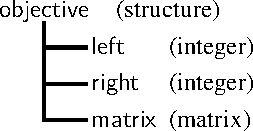
\includegraphics[scale=0.8]{../ch5/figures/objective}
\caption{Objective structure.}
\label{fig:struct:objective}
\end{subfigure}%
\begin{subfigure}{0.3\textwidth}
\centering
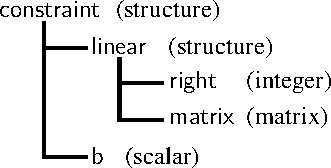
\includegraphics[scale=0.8]{../ch5/figures/constraint}
\caption{Constraint structure.}
\label{fig:struct:constraint}
\end{subfigure}%
\begin{subfigure}{0.3\textwidth}
\centering
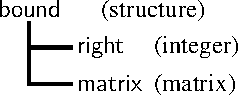
\includegraphics[scale=0.8]{../ch5/figures/bound}
\caption{Bound structure.}
\label{fig:struct:bound}
\end{subfigure}%

\caption{Structure definitions.}
\label{fig:struct}
\end{figure}

First, the structure definition in Fig.~\ref{fig:struct:objective} captures all of the objective terms outlined in Eqns.~(\ref{eq:ch5:QOFLagrange})--(\ref{eq:ch5:QOFMayer}).
The $\xvar{objective}$ structure is either $\mathcal{L}$ and $\mathcal{M}$ to account for Lagrange and Mayer terms, respectively.
Each entry in the structure is another term in the objective function.
The fields $\xvar{left}$ and $\xvar{right}$ can take on an integer value between $0$ and $5$, where $0$ indicates a singleton dimension (useful for linear and constant terms) and the remaining values correspond to the index of the expanded set of optimization variables introduced in Eqn.~(\ref{eq:ch5:varindices}).
Finally, $\xvar{matrix}$ is the potentially time-varying matrix of the appropriate size.
To illustrate this notation, consider the following LQ objective function: $\int_{t_0}^{t_f} \left[\sin(t) u_1^2(t) + \xi_2(t_0) \xi_1(t) \right] dt + \xi_1(t_f) -2 \xi_2(t_f)$.
The objective function can then be represented by the following\footnote{This example assumes $n_{\xi}=2$, $n_u=1$.}:%
\allowdisplaybreaks[1]%
\begin{subequations}%
\begin{align}
\int_{t_0}^{t_f}\sin(t) u_1^2(t)dt \ \Longleftrightarrow& \ \mathcal{L}\xind{1}.\xvar{left} = 1, \ \ \mathcal{L}\xind{1}.\xvar{right} = 1, \ \ \mathcal{L}\xind{1}.\xvar{matrix} = \sin(t) \\
% 
\int_{t_0}^{t_f}  \xi_2(t_0) \xi_1(t) dt \ \Longleftrightarrow& \ \mathcal{L}\xind{2}.\xvar{left} = 4, \ \ \mathcal{L}\xind{2}.\xvar{right} = 2, \ \ \mathcal{L}\xind{2}.\xvar{matrix} = \begin{bmatrix} 0 & 0 \\ 1 & 0 \end{bmatrix} \\
% 
\xi_1(t_f) -2 \xi_2(t_f) \ \Longleftrightarrow& \ \mathcal{M}\xind{1}.\xvar{left} = 0, \ \ \mathcal{M}\xind{1}.\xvar{right} = 5, \ \ \mathcal{M}\xind{1}.\xvar{matrix} = \begin{bmatrix} 1 \\ -2 \end{bmatrix}
\end{align}
\end{subequations}%
\allowdisplaybreaks[0]%

We now move onto the representation of the additional linear constraints in Eqns.~(\ref{eq:ch5:hqp})--(\ref{eq:ch5:gqp}).
The $\xvar{constraint}$ structure is either $\gls{Ycal}$ or $\gls{Zcal}$ to account for equality and inequality terms, respectively.
The field $\xvar{linear}$ can have multiple values to represent the summation needed for certain constraints.
The fields $\xvar{right}$ and $\xvar{matrix}$ are analogous to their use in the objective function terms.
The value for $\xvar{b}$ is the potentially time-varying function.
To illustrate this notation, consider the following linear constraints: $\xi_2(t_f) = 1$, $\xi_1(t) - 2 \xi_2(t) \leq 0$, and $u_1(t) - p_1 \leq \sin(t)$.
These linear constraints can then be represented by the following\footnote{This example assumes $n_{\xi}=2$, $n_u=1$, $n_p=1$.}:%
\allowdisplaybreaks[1]%
\begin{subequations}%
\small
\begin{align}
\xi_2(t_f) = 1 \ \Longleftrightarrow 
&\begin{cases}
\mathcal{Y}\xind{1}.\xvar{linear}\xind{1}.\xvar{right} = 5, \ \ \mathcal{Y}\xind{1}.\xvar{linear}\xind{1}.\xvar{matrix} = \begin{bmatrix} 0 \\ 1 \end{bmatrix}  \\
 \mathcal{Y}\xind{1}.\xvar{b} = 1 
\end{cases} \\
%
%
\xi_1(t) - 2 \xi_2(t) \leq 0 \ \Longleftrightarrow 
&\begin{cases}
\mathcal{Z}\xind{1}.\xvar{linear}\xind{1}.\xvar{right} = 2, \mathcal{Z}\xind{1}.\xvar{linear}\xind{1}.\xvar{matrix} = \begin{bmatrix} 1 \\ -2 \end{bmatrix} \\
\mathcal{Z}\xind{1}.\xvar{b} = 0 
\end{cases} \\
%
%
u_1(t) - p_1 \leq \sin(t) \ \Longleftrightarrow 
&\begin{cases}
\mathcal{Z}\xind{2}.\xvar{linear}\xind{1}.\xvar{right} = 1, \ \ \mathcal{Z}\xind{2}.\xvar{linear}\xind{1}.\xvar{matrix} = 1 \\
\mathcal{Z}\xind{2}.\xvar{linear}\xind{2}.\xvar{right} = 3, \ \ \mathcal{Z}\xind{2}.\xvar{linear}\xind{2}.\xvar{matrix} = -1 \\
\mathcal{Z}\xind{2}.\xvar{b} = \sin(t)
\end{cases}
\end{align}
\end{subequations}%
\allowdisplaybreaks[0]%

The $\xvar{bound}$ structure is used to represent additional linear constraints that can be written as simple upper and lower bounds as in Eqn.~(\ref{eq:ch5:simplebounds}).
Then the structure is either $\gls{UBcal}$ or $\gls{LBcal}$ to account for upper and lower terms, respectively.
The fields $\xvar{right}$ and $\xvar{matrix}$ are used analogously as the previous structures, with the exception that the values of $\xvar{matrix}$ can be $\pm \infty$ to indicate no bounds when appropriate.
To illustrate this notation, consider the following simple bounds: $u_1(t) \geq \sin(t)$ and $\xi_2(t) \leq \pi$.
Then these bounds can be represented by the following\footnote{This example assumes $n_{\xi}=2$, $n_u=1$.}:%
\begin{subequations}%
\begin{align}
u_1(t) \geq \sin(t) \quad \Longleftrightarrow& \quad \mathcal{LB}\xvar{\myind{1}.right} = 1, \quad \mathcal{LB}\xvar{\myind{1}.matrix} = \sin(t) \\
\xi_2(t) \leq \pi \quad \Longleftrightarrow& \quad \mathcal{UB}\xvar{\myind{1}.right} = 1, \quad \mathcal{UB}\xvar{\myind{1}.matrix} = \begin{bmatrix} \infty \\ \pi \end{bmatrix}
\end{align}
\end{subequations}%

%------------------------------------------------------------
\subsection{Procedure Overview}

A schematic overview of the \apgp{} is shown in Fig.~\ref{fig:overview}.
The user provides the problem structure using the notation defined in the previous section along with their choices for the mesh, quadrature, and defect constraints (these options are colored \textcolor{red}{red}).
These options are related to the acronyms used in Sec.~\ref{sec:ch5:formulation}.
We note that in addition to ED, LGL, and CGL mesh schemes, a user-defined mesh is also possible.
First, the mesh is generated and a number of initialization tasks are performed.
Next, the algorithms in the dashed box are presented in a modular format as the problem elements in \lqdo{} are separate, and are utilized only when necessary as they approximate specific problem elements.
Once all elements of the problem are approximated, the set of matrices that define the \qp{} are passed to an appropriate \qp{} solver to find the solution.

\tikzexternalexportnextfalse
\begin{figure}
\centering

\tikzstyle{block} = [rectangle, draw, fill=white, text centered, minimum height=2em, text width=9.5em]
\tikzstyle{block2} = [rectangle, draw, fill=white, text centered, minimum height=2em, text width=11.4em]
\tikzstyle{block3} = [rectangle, draw=red, text=red, fill=white, text centered, minimum height=2em, text width=5.5em]
\tikzstyle{block4} = [rectangle, draw=red, text=red, fill=white, text centered, minimum height=2em, text width=5.5em]
\tikzstyle{line} = [draw, -latex']
\tikzstyle{cloud} = [draw, ellipse,fill=white, node distance=3cm,
    minimum height=2em]

% \tikzset{every loop/.style={min distance=10mm,in=-185,out=-175,looseness=0}}

\tikzsetnextfilename{overview}
\resizebox{5in}{!}{%
\begin{tikzpicture}[
    pre/.style={>=latex',semithick},
    post/.style={>=latex,shorten >=1pt,>=latex',semithick,line width=1pt},
    mydouble/.style={<->, >=latex,shorten >=1pt,>=latex',semithick,line width=1pt},
    node distance = 3cm, auto
    ]
     
    \tikzset{
  manual input/.style={
    shape=trapezium,
    draw,
    shape border rotate=90,
    trapezium left angle=90,
    trapezium right angle=85}}

    % Place nodes
    
    % \node [] (solve) {solve};
    
    % \node [block, below=0.8cm of solve] (create) {create};
    \node [cloud] (create) {Problem structure};
    
    %
	\node [block, below=0.8cm of create] (initialize) {Initialize};
    
    \node [block2, right=0.8cm of initialize] (createT) {Create $\bm{t}$};
    
    \node [block3, manual input, above right=-0.4cm and 1.4cm of createT] (createTmethods) {\scriptsize ED, LGL, CGL, USER};
    
    %
	\node [block, below=0.8cm of initialize] (createH) {Hessian term \\ (see Alg.~\ref{alg:ch5:hessian})};
        
    %
	\node [block, below=0.8cm of createH] (createF) {Gradient term \\ ($\sim$ to Alg.~\ref{alg:ch5:hessian})};   
   
    %
	\node [block, below=0.8cm of createF] (createC) {Constant term \\ ($\sim$ to Alg.~\ref{alg:ch5:hessian})};  
    
	\node [block2, above right=-0.0cm and 0.8cm of createF] (Lbig) {$\mathcal{L}^{QP}$ terms (see Alg.~\ref{alg:ch5:Lterms})};
    
    \node [block3, manual input, above right=-0.4cm and 1.4cm of Lbig] (Lsmallmethods) {\scriptsize CEF, CTR, CQHS, G, CC};
    
	\node [block2, below right=-0.0cm and 0.8cm of createF] (Mbig) {$\mathcal{M}^{QP}$ terms (see Alg.~\ref{alg:ch5:Mterms})};
    

    %
	\node [block, below=0.8cm of createC] (createdefects) {Defect constraints \\ (see Algs.~\ref{alg:ch5:SSdefects}--\ref{alg:ch5:PSdefects})};
    
    \node [block4, manual input, right=3cm of createdefects] (Defectmethods) {\scriptsize ZOH, EF, TR, HS, RK4, PS};
    
    %
	\node [block, below=0.8cm of createdefects] (createYZ1) {Add. eq. constraints \\ (see Alg.~\ref{alg:ch5:constraints})};
    
    % \node [block2, above right=-0.43cm and 0.8cm of createYZ1] (path1) {$\bm{C}$ terms (see Alg.~\ref{})};
    
	% \node [block2, below right=-0.43cm and 0.8cm of createYZ1] (boundary1) {$\bm{\phi}$ terms (see Alg.~\ref{})};
    
    \node [block2, below right=-0.55cm and 0.8cm of createYZ1] (path) {$\bm{C}$ terms (see Alg.~\ref{alg:ch5:path})};
    
    %
	\node [block, below=0.8cm of createYZ1] (createYZ2) {Inequality constraints \\ (see Alg.~\ref{alg:ch5:constraints})};
    
    % \node [block2, above right=-0.43cm and 0.8cm of createYZ2] (path2) {$\bm{C}$ terms (see Alg.~\ref{})};
    
	% \node [block2, below right=-0.43cm and 0.8cm of createYZ2] (boundary2) {$\bm{\phi}$ terms (see Alg.~\ref{})};
       
	\node [block2, above right=-0.55cm and 0.8cm of createYZ2] (boundary) {$\bm{\phi}$ terms (see Alg.~\ref{alg:ch5:boundary})};
       
    \node [block, below=0.8cm of createYZ2] (createBnds) {Simple bounds \\ ($\sim$ to Alg.~\ref{alg:ch5:constraints})};
    
    \node [cloud, below=0.8cm of createBnds] (qpsolver) {To QP solver};
    
    \node [above right=-1.3cm and 1.4cm of qpsolver] (qp) {\begin{minipage}{0.3\textwidth}\textcolor{black!70}{
\begin{align*}
\min_{\mathbf{X}} \qquad& \frac{1}{2}\mathbf{X}\tran \mathbf{H} \mathbf{X} + \mathbf{F}\tran \mathbf{X} + c \\
\text{subject to:} \qquad& \begin{bmatrix} \mathbf{A}_{e1} \\ \mathbf{A}_{e2} \end{bmatrix}\mathbf{X} = \begin{bmatrix} \mathbf{B}_{e1} \\ \mathbf{B}_{e2} \end{bmatrix} \\
& \mathbf{A}_{i}\mathbf{X} \leq \mathbf{B}_{i} \\
& \myunderbar{\mathbf{X}} \leq \mathbf{X} \leq \myoverbar{\mathbf{X}} 
\end{align*}}
\end{minipage}};
    
    % outputs
	\node [left=0.8cm of createH] (outputH) {$\mathbf{H}$};
    
    \node [left=0.8cm of createF] (outputF) {$\mathbf{F}$};
    
    \node [left=0.8cm of createC] (outputC) {$c$};
    
    \node [left=0.8cm of createdefects] (outputdefects) {$\mathbf{A}_{e1}, \mathbf{B}_{e1}$};
    
    \node [left=0.8cm of createYZ1] (outputYZ1) {$\mathbf{A}_{e2}, \mathbf{B}_{e2}$};
    
    \node [left=0.8cm of createYZ2] (outputYZ2) {$\mathbf{A}_{i}, \mathbf{B}_{i}$};
    
    \node [left=0.8cm of createBnds] (outputBnds) {$\myunderbar{\mathbf{X}}$, $\myoverbar{\mathbf{X}}$};
    
    % boxes
	\node [dashed,  draw=black, minimum width=12em, minimum height=13.75cm, above=-13.5cm of createH] (method) {};
    
    % Draw edges
    \path [post, line] (createH) -- (outputH);
    \path [post, line] (createF) -- (outputF);
    \path [post, line] (createC) -- (outputC);
    \path [post, line] (createdefects) -- (outputdefects);
    \path [post, line] (createYZ1) -- (outputYZ1);
    \path [post, line] (createYZ2) -- (outputYZ2);
    \path [post, line] (createBnds) -- (outputBnds);
    
    % \path [post, line] (initialize) -- (createT);
    \path [mydouble, draw] (createT) -- (initialize);
    
    % \path [post, line] (createH.east) -- (Lbig.170);
    \path [mydouble, draw] (Lbig.175) -- (createH.east);
    
    % \path [post, line] (createH.east) -- (Mbig.170);
    \path [mydouble, draw] (Mbig.175) -- (createH.east);
    
    % \path [post, line] (createF.east) -- (Lbig.west);
    \path [mydouble, draw] (Lbig.west) -- (createF.east);
    
    % \path [post, line] (createF.east) -- (Mbig.west);
    \path [mydouble, draw] (Mbig.west) -- (createF.east);
    
    % \path [post, line] (createC.east) -- (Lbig.190);
    \path [mydouble, draw] (Lbig.185) -- (createC.east);
    
    % \path [post, line] (createC.east) -- (Mbig.190);
    \path [mydouble, draw] (Mbig.185) -- (createC.east);
        
    % \path [post, line] (createYZ1.east) -- (boundary.175);
    \path [mydouble, draw] (boundary.west) -- (createYZ1.east);
    
    % \path [post, line] (createYZ2.east) -- (boundary.185);
    \path [mydouble, draw] (boundary.west) -- (createYZ2.east);
    
    % \path [post, <->, line] (createYZ1.east) -- (path.175);
    \path [mydouble, draw] (path.west) -- (createYZ1.east);
    
    % \path [post, <->, line] (createYZ2.east) -- (path.185);
    \path [mydouble, draw] (path.west) -- (createYZ2.east);

   % \path [post, line] (Lbigmethods) -- (Lbig);
    
	\path [post, line] (Lsmallmethods.west) -- (Lbig.east);

    % \path [post, line] (Lsmallmethods.west) -- (Lsmall.east);
    
    % \path [post, line] (Lsmallmethods.west) -- (Lconstant.east);
    
    % \path [post, line] (Lconstantmethods) -- (Lconstant);
    
    \path [post, line] (Defectmethods.west) -- (createdefects.east);
    
    \path [post, line] (createTmethods.west) -- (createT.east);
    

\draw [decorate,decoration={brace,amplitude=10pt},xshift=-4pt,yshift=0pt]
(-3.3,-7.7) -- (-3.3,-3.2) node [black,midway,xshift=-0.3cm] 
{\footnotesize \rotatebox{90}{Objective function}};

\draw [decorate,decoration={brace,amplitude=10pt},xshift=-4pt,yshift=0pt]
(-4.4,-15.7) -- (-4.4,-9.1) node [black,midway,xshift=-0.3cm] 
{\footnotesize \rotatebox{90}{Constraints}};

% straight down
    \path [post, line] (create) -- (initialize);
    \path [post, line] (initialize.south) -- (method.north);
    \path [post, line] (method.south) -- (qpsolver.north);

\end{tikzpicture}
}
% \vspace{-0.3in}
\caption{Overview of the automated problem generation procedure.}\label{fig:overview}

\end{figure}

%------------------------------------------------------------
\subsection{Algorithms}

Here we briefly describe the algorithms with the full pseudocodes in Sec.~\ref{sec:app3:algorithms}.
The first algorithm outlines two functions used to get index sequence of the variable's location in both the continuous and discrete problems.
The function \textsc{GetContIndex} takes an integer between $0$ and $5$, used to denote a set of optimization variables in $\tilde{\bm{x}}$, and returns the sequence defining all the locations of that particular class of optimization variables in Eqn.~(\ref{eq:ch5:x:cont}).
The second function, \textsc{findQPindex}, requires three inputs: 1) \xvar{x} is the specific number of the optimization variable that is selected, 2) \xvar{xtype} is the same optimization variable classification as before, and 3) \xvar{idx} are the necessary indices to return.
For example, if $n_u = 2$, $n_{\xi} = 3$, and $n_{p} = 1$, then $\xvar{x}$ could be valued from $0$ to $6$ since there are $6$ total optimization variables.
Continuing with this example, if $\xvar{x} = 4$, $\xvar{xtype} = 2$, and $\xvar{idx} = 1 \text{ to } N_t$, then we are requesting the indices of the discretization of $\xi_2(t)$, i.e.,~$\mathbf{X}(\xvar{I}) = \xi_2(\bm{t})$.
Both of these functions will be useful when creating the objective function terms and additional linear constraints.

\subsubsection{Objective Function Terms} \label{sec:ch5:alg:objective}

There are three main algorithms are used to implement the five methods for approximating objective function terms in Sec.~\ref{sec:ch5:dt:objective}.
The Lagrange terms are approximated by quadrature in Alg.~\ref{alg:ch5:Lterms}.
The input is a structure $\mathcal{L}$ of type \xvar{objective} and for each substructure, the relevant sequences are created.
Both the \textsc{GetContIndex} and \textsc{GetQPIndex} are used to generate the appropriate row and column locations in the Hessian.
While the CQHS method is shown specifically, the other quadrature schemes can readily be implemented with the same pseudocode with modifications to lines \ref{line:ch5:V}--\ref{line:ch5:Voff} pertaining to the values of the diagonal and off-diagonal entries.
To visualize the process being used in Alg.~\ref{alg:ch5:Lterms}, the sparsity pattern for different $\bm{L}_{ij}$ is shown in Fig.~\ref{fig:figsparsityHSS}.
Each concatenation of \xvar{I} on line~\ref{line:ch5:lqp_I} in the algorithm is the addition of a single diagonal in Fig.~\ref{fig:figsparsityHSS}b or column in Fig.~\ref{fig:figsparsityHSS}d.

Compact and efficient formulas for the quadrature methods are achieved by the creation of $\xvar{H}$ (and similar terms) and the use of the $\textsc{rshift}$ function.
Consider the CTR method: 
\begin{align}
\begin{matrix}
\xvar{H} & =[& \Delta_0 & \Delta_1 & \cdots & \Delta_{n_t-1} & 0 &]  \\
\text{\textsc{rshift}}(\xvar{H}) & =[&  0 & \Delta_0 & \cdots & \Delta_{n_t-2} & \Delta_{n_t-1} &] \\
\xvar{Q} & =[&  \xvar{A}(t_0) & \xvar{A}(t_1) & \cdots & \xvar{A}(t_{n_t-1}) & \xvar{A}(t_{n_t})  &] \\
\text{CTR} & =[&  \Delta_0 \xvar{A}(t_0) & (\Delta_0+\Delta_1) \xvar{A}(t_1) & \cdots & (\Delta_{n_t-2}+\Delta_{n_t-1}) \xvar{A}(t_{n_t-1}) & \Delta_{n_t-1} \xvar{A}(t_{n_t}) &]
\end{matrix} 
\end{align}

\noindent We see the formula $\left( \xvar{H} \oplus \text{\textsc{rshift}}(\xvar{H}) \right)  \odot \xvar{Q}/2$ produces the appropriate entries for the CTR method in Eqn.~(\ref{eq:ch5:CTR}).

% new paragraph
The sequences for the Mayer terms are created with Alg.~\ref{alg:ch5:Mterms}, which is similar to the algorithm for the Lagrange terms.
The approximation of Mayer terms is the same across the quadrature methods as previously mentioned.

% new paragraph
To create the sparse Hessian matrix, Alg.~\ref{alg:ch5:hessian} takes the sequences from both Algs.~\ref{alg:ch5:Lterms}--\ref{alg:ch5:Mterms}.
The creation of the gradient and constant terms in Eqn.~(\ref{eq:ch5:qpH}) requires some minor modifications to Alg.~\ref{alg:ch5:hessian} but requires no modifications of Algs.~\ref{alg:ch5:Lterms}--\ref{alg:ch5:Mterms}. 

%------------------------------------------------------------
\subsubsection{Defect Constraints}

The algorithms for creating the defect constraints are shown in Alg.~\ref{alg:ch5:SSdefects} (SS methods) and Alg.~\ref{alg:ch5:PSdefects} (PS methods).
We will first describe the approach used for the SS methods based on Eqns.~(\ref{eq:ch5:ssdefects})--(\ref{eq:ch5:ssdefectsZOH}).
All required defect constraints for a particular state are generated inside the for-loop on line~\ref{line:ch5:SSdefects_for}.
In order, the appropriate entries in the matrix $\mathbf{A}_{e1}$ are generated for the controls, states, and parameters based on their $\bm{\theta}$ term expressions (see Eqn.~(\ref{eq:ch5:ss})).
The sparsity pattern for this matrix is shown in Fig.~\ref{fig:figsparsityASS}.
The row and column locations are generated through the appropriate sequences based on the number of variables and node points.
The values of the matrix entries are computed with element-wise formulas, similar to the approach used in the objective function terms (see Sec.~\ref{sec:ch5:alg:objective}).
The indexing vector $\xvar{T}$ allows us to extract matrix values on different time grids shifted by one index which are present due to the shifting of $k$ and $k+1$ values in the formulas.
Using this approach, all time-varying functions are evaluated only once on a particular time grid.

% new paragraph
The \textsc{kron} function\cite{matlab-kron} used on line~\ref{line:ch5:SSdefects_kron} generates a matrix that efficiently implements $\bm{I}$ in the equations (see its usage on lines~\ref{line:ch5:SSdefects_V1}--\ref{line:ch5:SSdefects_V2}).
For the states and controls, values are calculated for the lower and upper diagonals in their respective blocks.
For the controls, the lower diagonal values ($\bm{\theta}_1$ terms) are computed on line~\ref{line:ch5:SSdefects_V3} and the upper diagonal ($\bm{\theta}_2$ terms) are computed on the following line.
These diagonals are visualized in Figs.~\ref{fig:figsparsityASS}c--d.
Once the row, columns, and values for each state's defect constraints are generated, they are combined into a single sparse matrix of size $n_{\xi} n_t \times n_{X}$.
The disturbance in Eqn.~(\ref{eq:ch5:ss}) is the only part of the dynamics that appears in the $\mathbf{B}_{e1}$ term.
It is created in a similar fashion as the parameters (except there is only a single column in the resulting matrix).
The algorithm presented specifically implements the TR method, but can be readily adapted to the other SS methods (the formulas for \xvar{V} would need to be updated).

% new paragraph
For PS methods (both with LGL or CGL nodes) in Alg.~\ref{alg:ch5:PSdefects}, there is one more defect constraint per state than for an equivalent SS method.
Overall, the procedure is very similar to the one for SS methods.
The indexing vector $\xvar{T}$ is not needed since the matrix values only require the derivative function values at a single point in time in each row of the defect constraint (see the sparsity pattern in Figs.~\ref{fig:figsparsityAPS}b--d).
Instead of \xvar{K}, a PS method requires the differentiation matrix $\bm{D}$ to be provided.
This matrix is appropriately copied and shifted so that it coincides with the defect constraint rows and columns for the current state (see line~\ref{line:ch5:D}).
This is visualized with the block dense matrices in Fig.~\ref{fig:figsparsityAPS}a.

%------------------------------------------------------------
\subsubsection{Additional Linear Constraints and Bounds} \label{sec:ch5:alg:lin:constraints}

Both the additional inequality and equality constraints are created using Alg.~\ref{alg:ch5:constraints} taking in a structure of type $\textsf{constraint}$.
For each substructure (i.e.,~for each different constraint), we need to determine if its type is either path or boundary.
There are two conditions such that a constraint can be considered a path constraint: 1) any of the variable types in \textsf{right} are controls or states; 2) any of the matrices are time-varying (e.g.,~$\bm{Z}_3(t)$ or $\hat{Z}(t)$).

% new paragraph
If it is determined that the constraint is a path constraint, then Alg.~\ref{alg:ch5:path} is utilized to create the sparse matrix sequences.
Otherwise, Alg.~\ref{alg:ch5:boundary} is utilized.
These two algorithms are quite similar, the primary difference being how many constraints are created ($N_t$ vs. one).
Both utilize \textsc{GetContIndex} and \textsc{GetQPIndex} in a similar fashion to the objective function terms in Sec.~\ref{sec:ch5:alg:objective}.
After all sequences are created and combined, the sparse matrix is generated.

% new paragraph
For simple bounds in Eqn.~(\ref{eq:ch5:simplebounds}), the \textsf{bound} structure type is used.
The same algorithms are applicable but the entries are initialized as either $-\infty$ or $\infty$ depending on if it is a lower or upper bound.
This ensures that unconstrained variables remain unconstrained.

%-------------------------------------------------------------------
\section{Extensions} \label{sec:ch5:extensions}

In this section, a number of extensions are described that still fit under the \lqdo{} problem form using either some type of transformation or a simple application of the \apgp.

%-----------------------------------------------------------
\subsection{Integral Constraints} \label{sec:ch5:integral:constraints}

Due to the equivalence between $\mathcal{L}$ and $\mathcal{M}$, frequently the integral part of Eqn.~(\ref{eq:ch5:NLobj}) is converted to an equivalent dynamic constraint \cite{Bryson1975a, Betts2010a, Stryk1999a}. 
Since the dynamic constraints are linear in \lqdo, there can only be integral terms with a linear dependence. 
Therefore, we cannot utilize the transformation with quadratic objective terms and still have a \qp.
However we still can use this transformation if linear integral constraints are present.
Consider the following inequality integral constraint \cite{Stryk1999a}:
\begin{align}
\int_{t_0}^{t_f} \left[ \bm{I}\tran(t) \tilde{\bm{x}} \right] dt - \hat{I} \leq  0
\end{align}

\noindent where $\gls{Ib}(t)$ is the integral matrix and $\hat{I}$ is a scalar. We can add an equivalent state $\xi_{n_{\xi}+1} := \xi_{\glsfirst{additional}}$ that has the same rate of change:
\begin{align}
\dot{\xi}_+ = \bm{I}\tran(t) \tilde{\bm{x}}
\end{align}

\noindent Then we add the following initial value equality and final value inequality constraints:
\begin{align}
\xi_+(t_0) = 0, \quad \xi_+(t_f) \leq \hat{I} 
\end{align}

\noindent An similar procedure can be used for an equality constraint and additional states can be added for each linear integral constraint present in the problem.

%-----------------------------------------------------------
\subsection{Min-Max Objectives} \label{sec:ch5:minmax:objective}

A min-max objective function for Prob.~(\ref{eq:ch5:NLDO}) has the form \cite{Stryk1999a}:
\begin{align}
\Psi = \min_{\bm{x}} \max_{t\in[t_0,t_f]} \mathcal{E}\big(t, \bm{\xi}(t), \bu(t), \bp, t_0, \bm{\xi}(t_0), t_f, \bm{\xi}(t_f) \big)
\end{align}

\noindent where $\gls{extremum}$ is the extremum function.
We can introduce an additional parameter $p_{n_p+1} := p_+$ to transform this min-max problem into Mayer form by introducing an additional inequality constraint:
\begin{align}
\mathcal{E}\big(t, \bm{\xi}(t), \bu(t), \bp, t_0, \bm{\xi}(t_0), t_f, \bm{\xi}(t_f) \big) - p_+ \leq 0
\end{align}

\noindent and modifying the objective to:
\begin{align}
\min_{\bm{x}, p_+}\ p_+
\end{align}

This type of transformation is one of the common uses of parameters in \lqdo{} problems assuming the extremum function is of the appropriate form.
This appropriate form of $\mathcal{E}$ (linear terms) was already discussed in Sec.~\ref{sec:ch5:integral:constraints} as we are transforming part of the objective to Mayer form.
The structure of this transformation also allows for the extremum function to consist of multiple expressions such as the following:
\begin{align}
\min_{\bm{x}} \max_{t\in[t_0,t_f]}\ \{ u_1(t), \xi_1(t) + \xi_2(t) \}
\end{align}

\noindent which would be approximated with two additional constraints using the same parameter (i.e.,~$u_1(t) - p_+ \leq 0$ and $\xi_1(t) + \xi_2(t) - p_+ \leq 0$).
The requirement only is that each expression in the maximization can be properly written as a linear inequality constraint bounded by the additional parameter.

%-----------------------------------------------------------
\subsection{Absolute Values in the Objective (and Constraints)} \label{sec:ch5:absolute:values}

Consider the following finite-dimensional optimization problem:%
\begin{subequations} \label{eq:ch5:absolute}
\begin{align} 
\min_{\bm{z}_1, \bm{z}_2 } \quad &\abs*{\mathcal{F}_1(\bm{z}_1)} + \mathcal{F}_2(\bm{z}_2) \label{eq:ch5:absolute_obj} \\
\text{subject to:} \quad & \bm{g}(\bm{z}_1, \bm{z}_2, \abs*{\mathcal{F}_1(\bm{z}_1)}) \leq \bm{0}
\end{align}
\end{subequations}%

\noindent Since the absolute value term is being minimized and contains a distinct set of the optimization variables, we can add an additional parameter $p_{n_p+1} := p_+$ and two inequality constraints to arrive at the following equivalent problem:%
\begin{subequations}%
\begin{align}
\min_{\bm{z}_1, \bm{z}_2, p_+} \quad & p_+ + \mathcal{F}_2(\bm{z}_2) \\
\text{subject to:} \quad & \bm{g}(\bm{z}_1, \bm{z}_2, p_+ ) \leq \bm{0} \\
& \mathcal{F}_1(\bm{z}_1) - p_+ \leq 0 \\
& -\mathcal{F}_1(\bm{z}_1) - p_+ \leq 0
\end{align}
\end{subequations}%

\noindent An alternative reformulation utilizes the sum of two positive parameters for the absolute value. % maybe reference?
As with the previous two extensions, this extension introduces additional constraints that are linear with respect to the added parameter; so as long as $\mathcal{F}_1$ is linear, the additional constraints will be linear.
For example, $\min\ \abs{\xi_1(t_f) + \xi_2(t_f)}$.
We can also have $\mathcal{F}_1$ in the Lagrange term, i.e.,~$ \int_{t_0}^{t_f} \abs*{\mathcal{F}_1} dt$.
Recall that the quadrature approximations for linear terms for all the methods in Sec.~\ref{sec:ch5:dt:objective} are the sum of the products of a positive step size (or weight) and the value at every node point.
Therefore, each point in the quadrature approximation is in the form of Eqn.~(\ref{eq:ch5:absolute_obj}).
However, we now need a parameter for each point in time to accurately capture that integral behavior.
An example objective is $\min \ \int_{t_0}^{t_f} \abs{u_1(t)} dt$.

Absolute value constraints with linear terms can readily be handled as well if they form a convex feasible region. % potentially add a reference
For example, $\abs{\xi_1(t) + \xi_2(t)} \geq 1$ would not be convex.

%-----------------------------------------------------------
\subsection{Output Tracking} \label{sec:ch5:output}

Tracking a reference signal, either a set point or reference trajectories, can be a critical measure for control-system performance \cite{Bryson1975a, Anderson2007a}.
Generally, the tracking error in the reference is computed against an output signal of the following form:
\begin{align}
\gls{output}(t) = \gls{Cb}(t) \bm{\xi}(t) + \gls{Db}(t) \bm{u}(t)  + \gls{Vb}(t) \bm{p} + \bm{E}(t)\bm{d}(t)
\end{align}

\noindent where $\{\bm{C}, \bm{D}, \bm{V}, \bm{E}\}$ are the LTV output matrices.
The output equation is similar to the dynamics in Eqn.~(\ref{eq:ch5:fdyn}), but no derivatives appear.
Let us denote the reference signals as $\tilde{\bm{y}} = \tilde{\bm{y}}(t)$, then a suitable output tracking error quadratic objective function is:
\begin{gather} \Psi =  \int_{t_0}^{t_f} \left[ \left( \bm{y} - \tilde{\bm{y}} \right)\tran \bm{O}(t) \left( \bm{y} - \tilde{\bm{y}} \right) \right] dt
\end{gather}

\noindent where $\gls{Out}$ is a symmetric weighting matrix. This objective function can be put into the same form as Eqn.~(\ref{eq:ch5:QOFLagrange}):%
\begin{subequations}
\begin{gather} \Psi \equiv \int_{t_0}^{t_f} \left[ \bm{x}\tran \bm{L}_{\glsfirst{notoutput}} \bm{x} + \bm{l}_{O}\tran \bm{x} + c_O\right] dt \\
\text{where:} \qquad 
\bm{L}_{O} = \begin{bmatrix}
\bm{C}\tran \bm{O} \bm{C} & \bm{C}\tran \bm{O} \bm{D} & \bm{C}\tran \bm{O} \bm{V} \\
\bm{D}\tran \bm{O} \bm{C} & \bm{D}\tran \bm{O} \bm{D} & \bm{D}\tran \bm{O} \bm{V}   \\
\bm{V}\tran \bm{O} \bm{C} & \bm{V}\tran \bm{O} \bm{D} & \bm{V}\tran \bm{O} \bm{V}   \\
\end{bmatrix} \\
\bm{l}_{O}\tran =  \left( 2 \tilde{\bm{y}}\tran \bm{O} + 2\bm{d}\tran \bm{E}\tran \bm{O} \right) \begin{bmatrix} \bm{C} \\ \bm{D} \\ \bm{V} \end{bmatrix}\tran, \quad 
c_O = \tilde{\bm{y}}\tran \bm{O} \tilde{\bm{y}} + \tilde{\bm{y}}\tran \bm{O} \bm{E} \bm{d}
\end{gather}
\end{subequations}%

\noindent Therefore, output tracking can be easily incorporated into the previous quadratic objective. 
Bryson and Ho provide a \glsfoo[noindex]{BVP} solution to a simpler output tracking problem \cite{Bryson1975a}.

%-----------------------------------------------------------
\subsection{Higher-Order Differential Equations} \label{sec:ch5:higher:order}

Equation~(\ref{eq:ch5:fdyn}) is a first-order linear differential equation. 
In general, there may be higher-order derivatives present.
Consider the following third-order differential equation with $E_3(t) \neq 0$:
\begin{align}
E_3(t)\dddot{\xi}_1+ E_2(t)\ddot{\xi}_1 + E_1(t)\dot{\xi}_1 = A(t)\xi_1 + B(t) u
\end{align}

\noindent To convert this into a first-order differential equation, we can add an additional state for each higher-order derivative present \cite{Stryk1999a}.
The dynamics of these state variables will be state of one order less.
For the example above, we would have:
\begin{align}
\begin{bmatrix}
\dot{\xi}_1 \\ \dot{\xi}_2 \\ \dot{\xi}_3
\end{bmatrix}
=
\begin{bmatrix}
0 & 1 & 0 \\
0 & 0 & 1 \\
\nicefrac{A}{E_3} & \nicefrac{-E_1}{E_3} & \nicefrac{-E_2}{E_3} \\
\end{bmatrix}
\begin{bmatrix}
\xi_1 \\ \xi_2 \\ \xi_3
\end{bmatrix}
+ 
\begin{bmatrix}
 0 \\ 0 \\ \nicefrac{B}{E_3}
\end{bmatrix} u
\end{align}

\noindent which is in the form of $\bm{f}^{QP}$ and therefore, these types of higher-order differential equations can be readily handled by \lqdo{}.

%-----------------------------------------------------------
\subsection{Control Rate Constraints}

In some problems, we want to include the rate at which the control changes $\dot{u}$ in our objective function or as a constraint such as \cite{Biegler2010a}:
\begin{align}
\dot{u}(t) \leq \dot{u}_{\max}
\end{align}

\noindent This situation can be handled in a similar manner as the higher-order differential equations in Sec.~\ref{sec:ch5:higher:order}.
We treat the control as another state variable $\xi_{n_\xi+1} := \xi_+ = u$ with dynamics of $\dot{\xi}_+ = \dot{u}$.
Now $\dot{u}$ is the independent input the system.
Both $u$ and $\dot{u}$ can be naturally handled using path constraints, objective function terms, etc.
This transformation also works with higher-order control derivatives such as $\ddot{u}$.

%-----------------------------------------------------------
\subsection{Polyhedra Constraints} \label{sec:ch5:polyhedra}

A common constraint in convex optimization is that the optimization variables must lie in some convex region.
In general, this region cannot be directly handled in \lqdo{}, but an approximation can be constructed with a polyhedron using the convex hull of a finite set of points on the region's boundary.
This polyhedron is characterized by a set of linear inequality constraints and any point that is found to be feasible in the polyhedron would be feasible in the original region.
An example is $u_1^2(t) + u_2^2(t) \leq 1$, which is an elliptical region that can be approximated (see Ref.~\cite{matlab-elliptical}).
Each additional linear constraint would be either a boundary or path constraint, so they would greatly add to the total number of constraints.
Polyhedral regions are also used in piecewise affine systems (systems with different dynamics depending on the specific location in the state-input space) \cite{Borrelli2015a}.

%-----------------------------------------------------------
\subsection{Bilevel Optimization and Minimum Time Problems} \label{sec:ch5:mtp}

Bilevel optimization is where one optimization problem is embedded (nested) within another \cite{Colson2007a}.
In some problems, the embedded problem has the form of \lqdo, such as some nested co-design problem formulations as was discussed in Chapter~\ref{ch:3} \cite{Herber2017b, Chilan2017a}.
For example, the outer loop may consist of variables that modify the matrices such as $\bm{A}$ and $\bm{B}$ (see Chapters~\ref{ch:7} and \ref{ch:8} for examples that use \lqdo{} and the \apgp{} on a problem with this property).

Minimum time problems directly include $t_0$ and $t_f$ in the objective function.
For example, if $\mathcal{M} = t_f$, then it might seem possible to treat $t_f$ as an optimization variable and have a linear term in the objective function.
However, treating $t_f$ as an optimization variable results in nonlinear defect constraints and $\mathcal{L}$ approximations.
Observing Eqn.~(\ref{eq:ch5:defect:PS}) and Eqn.~(\ref{eq:ch5:ssdefects}), we see direct dependence on $\Delta$ in the defect constraint formulas.
Therefore, minimum time problems \textit{cannot} be solved directly with a \qp.
One solution approach for minimum time problems that still uses the \lqdo{} framework is to solve a bilevel (nested) optimization problem.
The outer loop solves the single variable problem optimization for $t_f$ with the \qp{} formulation (for a fixed value of $t_f$) as the inner-loop solution.
If we expand to quadratically-constrained {\qp}s (see Sec.~\ref{sec:ch5:QCQP}), we can directly represent some minimum time problems.

%-----------------------------------------------------------
\subsection{Use in Nonlinear Optimal Control Problems}

In some problems, there might be a quadratic objective but nonlinear dynamics or a nonlinear objective and linear dynamics.
If certain problem elements fit the \lqdo{} form, then the appropriate matrices can be generated (recall Fig.~\ref{fig:overview} where the algorithms for generating the \qp{} matrices are modular).
These matrices then can be combined with the nonlinear elements of the problem and solved with nonlinear programming solvers.
Many of these solvers have special categorizations in order to efficiently leverage the problem structure such as for linear equality or inequality constraints.

%-------------------------------------------------------------------
\section{Numerical Examples} \label{sec:ch5:examples}

In this section, we will use five numerical examples to demonstrate the efficacy of the proposed \apgp.
The first four examples have known solutions that can be used to compute the optimal trajectories and objective function value to high precision.
Therefore, we can directly compare the different solution methods based on their deviation from the known solution.
The errors are reported as local maximum/minimum values (i.e.,~as a forward-looking moving maximum/minimum) in order to discuss the converge behavior independent of fortuitous meshes (e.g.,~the nodes points happen to be exactly at the time value where a path constraint should change activity).
In addition to comparing the absolute error, we will look at the time to create the \qp{} with the \apgp{} and the total \qp{} time (creation plus solver time).
Other performance metrics include local and global error, robustness to initial guess\footnote{The chosen solver does not require an initial guess.}, and problem size or memory needed \cite{Williams2005a, Wang2009a}.
Please see Refs.~\cite{Williams2005a, Wang2009a, Faedo2017a} for numerical comparisons between some of the \dt{} methods.
It remains future work to perform these additional comparisons.

% new paragraph
All tests were performed on a personal computer with an i7-6800K at 3.8 GHz (up to 12 threads available), 32 GB DDR4 3200 MHz RAM, \textsc{Windows} 10 64-bit, and \textsc{Matlab} 2017a.
The \qp{} solver used was the standard solver \textsc{quadprog} in \textsc{Matlab} using the \xvar{interior-point-convex} algorithm \cite{matlab-quadprog}.
All tolerances were set to $10\epsilon$, where $\epsilon$ is the machine precision number, in order to obtain the best solution possible for a particular \qp.
The complete set of codes from the \apgp{} and examples are available at Ref.~\cite{github-dt-qp-project}.

%-------------------------------------------------------------
\subsection{Example 1} \label{sec:ch5:example1}

%-------------------------------------------------------------
\subsubsection{Description}

For the first example, we will consider the problem on pp.~166--167 from Ref.~\cite{Bryson1975a}:%
\begin{subequations}%
\begin{align}
\min_{u(t)} \quad & \frac{1}{2}\int_0^{t_f} u^2 dt \\
\text{subject to:} \quad & \dot{\bm{\xi}} = \begin{bmatrix} 0 & 1 \\ -1 & 0 \end{bmatrix} \bm{\xi} + \begin{bmatrix} 0 \\ 1 \end{bmatrix} u \\
& {\xi}_1(0) = x_0, \quad {\xi}_2(0) = v_0, \quad {\xi}_1(t_f) = 0, \quad {\xi}_2(t_f) = 0
\end{align} 
\end{subequations}%

\noindent Although there are no path constraints, both the initial and final state values are fully constrained. 
As a result, this problem does not fit many traditional \lqdo{} problem definitions such as Prob.~(\ref{eq:ch5:lqr}).
The structure-based problem description for this example is:%
\allowdisplaybreaks[1]%
\begin{subequations}%
\begin{gather}
% Lagrange term
\mathcal{L}\xind{1}.\xvar{left} = 1, \quad \mathcal{L}\xind{1}.\xvar{right} = 1, \quad \mathcal{L}\xind{1}.\xvar{matrix} = 1/2 \\
% system dynamics
\bm{A} = \begin{bmatrix} 0 & 1 \\ -1 & 0 \end{bmatrix}, \quad \bm{B} = \begin{bmatrix} 0 \\ 1 \end{bmatrix} \\
% linear equality constraints
\mathcal{LB}\xind{1}.\xvar{right} = 4, \quad \mathcal{LB}\xind{1}.\xvar{matrix} = \begin{bmatrix} x_0 & v_0 \end{bmatrix}\tran \\
\mathcal{LB}\xind{2}.\xvar{right} = 5, \quad \mathcal{LB}\xind{2}.\xvar{matrix} = \begin{bmatrix} 0 & 0 \end{bmatrix}\tran \\
\mathcal{UB}\xind{1}.\xvar{right} = 4, \quad \mathcal{UB}\xind{1}.\xvar{matrix} = \begin{bmatrix} x_0 & v_0 \end{bmatrix}\tran \\
\mathcal{UB}\xind{2}.\xvar{right} = 5, \quad \mathcal{UB}\xind{2}.\xvar{matrix} = \begin{bmatrix} 0 & 0 \end{bmatrix}\tran
\end{gather} 
\end{subequations}%
\allowdisplaybreaks[0]

\noindent The \textsc{Matlab} code is in Sec.~\ref{sec:ex1-code}.

%-------------------------------------------------------------
\subsubsection{Solution}

\begin{figure}
\centering

\begin{subfigure}{0.5\textwidth}
\centering
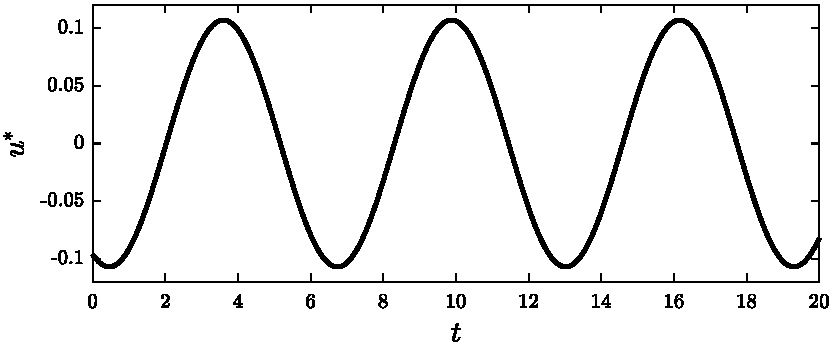
\includegraphics[width=\textwidth]{../ch5/figures/ex1sol-controls}%
\caption{Control.}
\label{fig:ch5:ex1sol:controls}
\end{subfigure}%
\begin{subfigure}{0.5\textwidth}
\centering
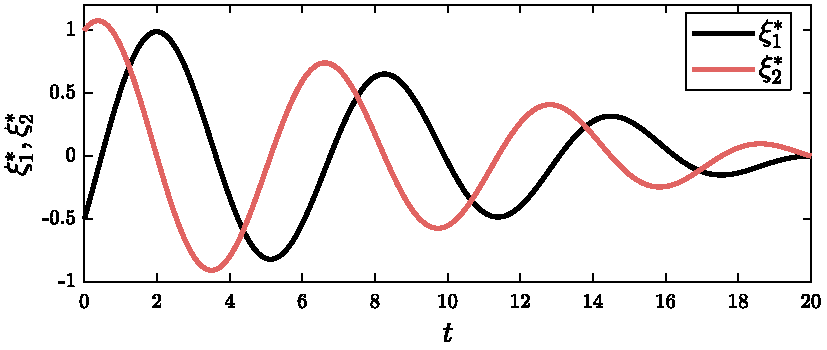
\includegraphics[width=\textwidth]{../ch5/figures/ex1sol-states}%
\caption{States.}
\label{fig:ch5:ex1sol:states}
\end{subfigure}%

\caption{Solution for \nameref{sec:ch5:example1}.}
\label{fig:ch5:ex1sol}
\end{figure}

It can be shown that the control trajectory that minimizes the objective while satisfying the constraints is:
\begin{align}
u^{\glsfoo[noindex]{optimal}}(t) = -\frac{2}{t_f^2 - \sin^2(t_f)}
\begin{bmatrix}
x_0 \\ v_0 
\end{bmatrix}\tran
\begin{bmatrix}
\sin(t_f -t) \sin(t_f) - t_f \sin(t) \\
-\cos(t_f -t) \sin(t_f) + t_f \cos(t)
\end{bmatrix}
\end{align}

\noindent with an optimal objective function value of:
\begin{align}
\Psi^* = \frac{t_f \left({v_{0}}^2+{x_{0}}^2\right)+2 {t_f}^2 v_{0} x_{0}-\cos\left(t_f\right) \sin\left(t_f\right) \left({v_{0}}^2-{x_{0}}^2\right)}{{{t_f}^2 - \sin\left(t_f\right)}^2} -2 v_{0} x_{0}
\end{align}

\noindent The problem parameters used are $t \in [0, 20]$, $x_0 = -1/2$, and $v_0 = 1$.
With these parameter values, $\Psi^* = 0.059842$.
The optimal trajectories for both the control and states is shown in Fig.~\ref{fig:ch5:ex1sol}.

%-------------------------------------------------------------
\subsubsection{Numerical Results}

% (convergence)
The convergence results for the eight tested schemes are shown in Fig.~\ref{fig:ch5:ex1sens:objective} (objective) and Fig.~\ref{fig:ch5:ex1sens:control} (controls).
The best scheme in terms of overall convergence rate was LGL-PS-G (7), and it is nearly linear.
However, once the scheme's accuracy was near machine epsilon, an accuracy threshold was reached and even started to slowly diverge (perhaps due to small errors in the calculation of the differentiation matrix, weights, etc.).
The next best scheme was CGL-PS-CC (8). 
It seemed to have a similar convergence rate as the other PS-based scheme, but it eventually achieves a sublinear rate of convergence until it reaches the precision threshold (for the objective value).

The SS-based schemes now remain. The best was ED-HS-CQHS (5), although ED-RK4-CQHS (6) was only slightly worse.
These are the two schemes that utilize the proposed CQHS quadrature method.
The convergence rate seemed to be sublinear, and an objective value accuracy threshold was reached for both schemes.
The control error between these schemes was nearly identical.
Next, perhaps surprisingly, was ED-ZOH-CEF (1).
Even though this scheme assumed piecewise constant control, it performed better than some of the more classical SS-based schemes.
Some of this accuracy may be due to the exact approximation of the objective function (i.e.,~only $u^2$ terms). 
ED-HS-CTR (4) was slightly better than ED-TR-CTR (3), indicating that the higher-order HS method did indeed provide additional accuracy for the same number of nodes.
Finally, ED-ZOH-CEF (1) was the worst scheme tested.

\begin{figure}%
\centering

{\footnotesize Local maximum values (local minimum values are in a thinner, translucent color):}


\includegraphics[width=\textwidth]{../ch5/figures/ex1_sens_legend}%

\vspace{1mm}

\begin{subfigure}{0.5\textwidth}
\centering
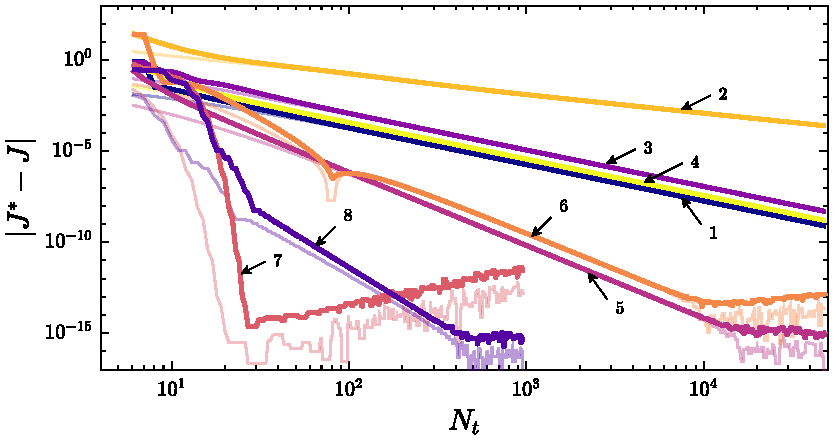
\includegraphics[width=\textwidth]{../ch5/figures/ex1_sens_objective}%
\caption{Objective error.}
\label{fig:ch5:ex1sens:objective}
\end{subfigure}%
\begin{subfigure}{0.5\textwidth}
\centering
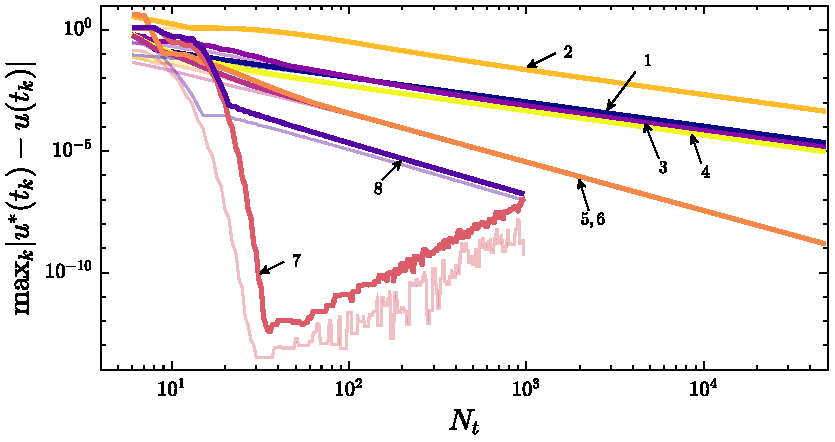
\includegraphics[width=\textwidth]{../ch5/figures/ex1_sens_control}%
\caption{Control error.}
\label{fig:ch5:ex1sens:control}
\end{subfigure}%

\begin{subfigure}{0.5\textwidth}
\centering
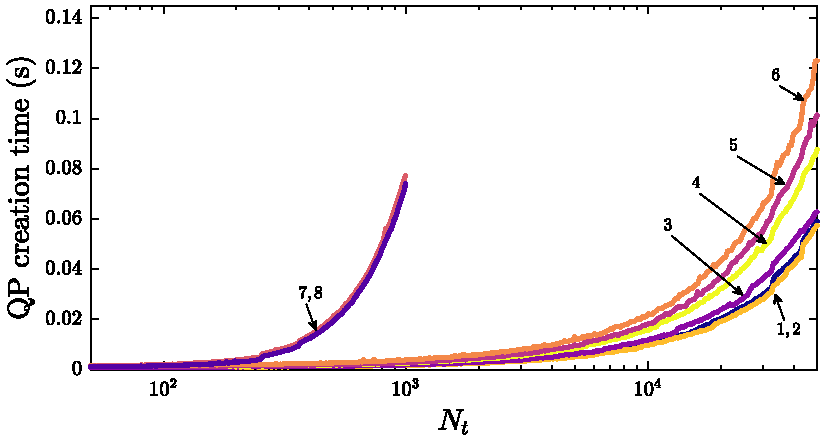
\includegraphics[width=\textwidth]{../ch5/figures/ex1_sens_qp_time}%
\caption{\qp{} creation time vs. $N_t$.}
\label{fig:ch5:ex1sens:qptime}
\end{subfigure}%
\begin{subfigure}{0.5\textwidth}
\centering
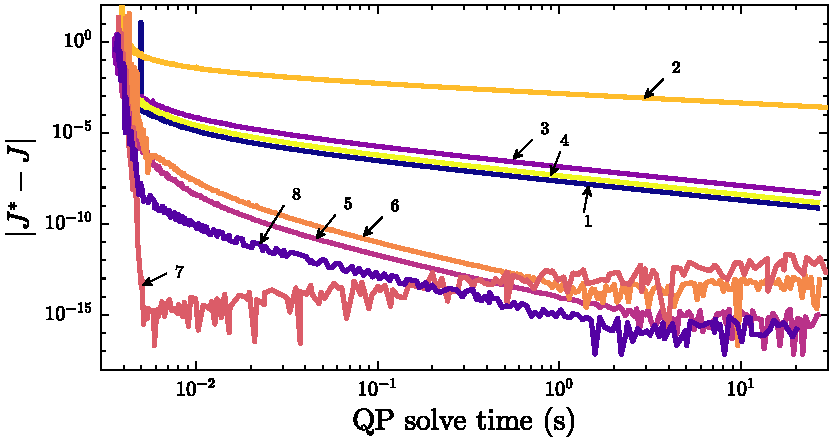
\includegraphics[width=\textwidth]{../ch5/figures/ex1_sens_solve_time}%
\caption{Objective error vs. total \qp{} solve time.}
\label{fig:ch5:ex1sens:solvetime}
\end{subfigure}%

\caption{Numerical results for \nameref{sec:ch5:example1}.}
\label{fig:ch5:ex1sens}
\end{figure}%

% new paragraph (qp creation time)
The time to create the \qp{} vs.~$N_t$ for each scheme is shown in Fig.~\ref{fig:ch5:ex1sens:qptime}.
Here we see two distinct groups: one for the PS-based schemes, and one for the SS-based schemes.
The PS-based schemes take a longer amount of time for a specific $N_t$ because the sparse matrices are much denser (cf. Fig.~\ref{fig:figsparsityAPS} and Fig.~\ref{fig:figsparsityASS}).
The primary cost is the construction of the sparse matrices from the sequences.
The SS-based schemes do vary in their creation time with the schemes, with more matrix calculations and denser defect constraint matrices being slower to create.
Therefore, we observe that (1) is the fastest and (6) is the slowest.
All creation times for this problem are under 0.13~s, even for larger $N_t$.

% new paragraph (qp solve time)
A fairer comparison between the schemes considers the tradeoffs between accuracy and total solve time.
The time to create and solve the \qp{} vs. the error in the objective function is shown in Fig.~\ref{fig:ch5:ex1sens:solvetime}.
The ordering is generally the same as the error plots, and (7) is clearly the preferred scheme for this problem.
Schemes (5) and (6) are slightly more attractive as the computation time for a given error is only slightly slower than the PS-based schemes.

%-------------------------------------------------------------
\subsection{Example 2} \label{sec:ch5:example2}

%-------------------------------------------------------------
\subsubsection{Description}
For the second example, we will consider the problem on pp.~120--122 from Ref.~\cite{Bryson1975a} and in Ref.~\cite{Bryson1963a}:
\begin{subequations}%%
\begin{align}
\min_{u} \quad & \frac{1}{2}\int_{0}^{1} u^2 dt \\
\text{subject to:} \quad  & \dot{\bm{\xi}} = \begin{bmatrix} \xi_2 \\ u \end{bmatrix} \\
& \xi_1(0) = 0, \quad \xi_1(1) = 0, \quad \xi_2(0) = 1, \quad \xi_2(1) = -1 \\
& \xi_1(t) \leq \ell
\end{align}
\end{subequations}%

\noindent This problem is similar to \nameref{sec:ch5:example1} but, now has a path constraint.
The structure-based problem description for this example is:%
\allowdisplaybreaks[1]
\begin{subequations}%
\begin{gather}
% Lagrange term
\mathcal{L}\xind{1}.\xvar{left} = 1, \quad \mathcal{L}\xind{1}.\xvar{right} = 1, \quad \mathcal{L}\xind{1}.\xvar{matrix} = 1/2 \\
% system dynamics
\bm{A} = \begin{bmatrix} 0 & 1 \\ 0 & 0
\end{bmatrix}, \quad \bm{B} = \begin{bmatrix} 0 \\ 1
\end{bmatrix} \\
% linear equality constraints
\mathcal{LB}\xind{1}.\xvar{right} = 4, \quad \mathcal{LB}\xind{1}.\xvar{matrix} = \begin{bmatrix} 0 & 1 \end{bmatrix}\tran \\
\mathcal{LB}\xind{2}.\xvar{right} = 5, \quad \mathcal{LB}\xind{2}.\xvar{matrix} = \begin{bmatrix} 0 & -1 \end{bmatrix}\tran \\
\mathcal{UB}\xind{1}.\xvar{right} = 4, \quad \mathcal{UB}\xind{1}.\xvar{matrix} = \begin{bmatrix} 0 & 1 \end{bmatrix}\tran \\
\mathcal{UB}\xind{2}.\xvar{right} = 5, \quad \mathcal{UB}\xind{2}.\xvar{matrix} = \begin{bmatrix} 0 & -1 \end{bmatrix}\tran \\
\mathcal{UB}\xind{3}.\xvar{right} = 2, \quad \mathcal{UB}\xind{3}.\xvar{matrix} = \begin{bmatrix}\ell & \infty \end{bmatrix}\tran % \\
\end{gather}
\end{subequations}%%
\allowdisplaybreaks[0]%

\noindent The \textsc{Matlab} code is in Sec.~\ref{sec:ex2-code}.

%-------------------------------------------------------------
\subsubsection{Solution}

\begin{figure}
\centering

\begin{subfigure}{0.5\textwidth}
\centering
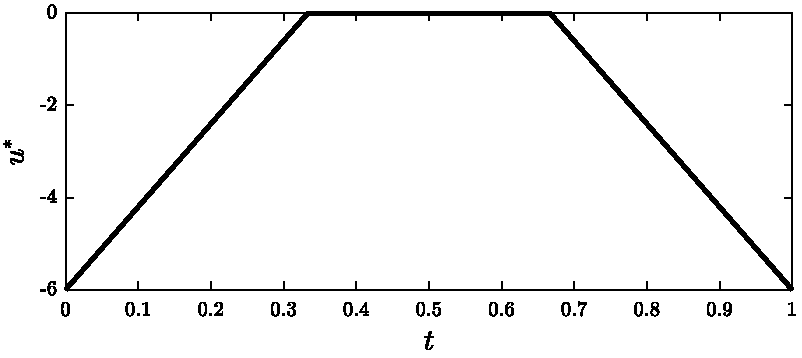
\includegraphics[width=\textwidth]{../ch5/figures/ex2sol-controls}%
\caption{Control.}
\label{fig:ch5:ex2sol:controls}
\end{subfigure}%
\begin{subfigure}{0.5\textwidth}
\centering
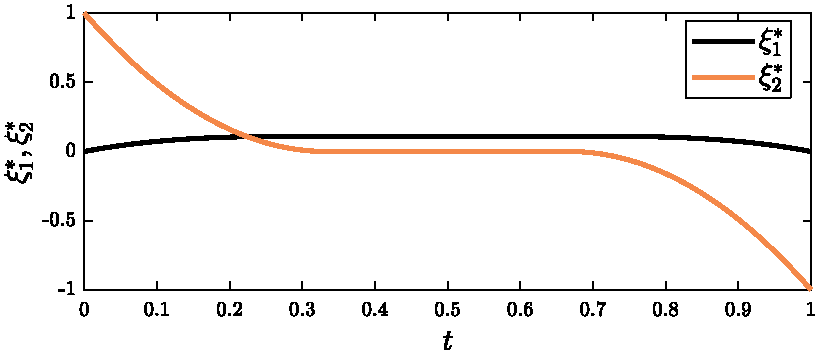
\includegraphics[width=\textwidth]{../ch5/figures/ex2sol-states}%
\caption{States.}
\label{fig:ch5:ex2sol:states}
\end{subfigure}%

\caption{Solution for \nameref{sec:ch5:example2}.}
\label{fig:ch5:ex2sol}
\end{figure}

It can be shown that the control trajectory that minimizes the objective while satisfying the constraints when $0 < \ell \leq 1/6$ is:
\begin{align}
u^*(t) = \begin{cases}
-\frac{2}{3\ell}\left( 1 - \frac{t}{3\ell} \right) & 0 \leq t < 3\ell \\
0 & 3\ell \leq t < 1 - 3\ell \\
-\frac{2}{3\ell}\left( 1 - \frac{1-t}{3\ell} \right) & 0 \leq t \leq 3\ell \\
\end{cases}
\end{align}

\noindent with an optimal objective function value of:
\begin{align}
\Psi^* = \frac{4}{9\ell}
\end{align}

\noindent A problem parameter value of $\ell = 1/9$ will be used, and with this value, $\Psi^* = 4$.
The optimal trajectories for both the control and states are shown in Fig.~\ref{fig:ch5:ex2sol}.

%-------------------------------------------------------------
\subsubsection{Numerical Results}

The convergence results for the eight tested schemes are shown in Fig.~\ref{fig:ch5:ex2sens}.
All schemes, including the PS-based schemes, achieve similar sublinear convergence rates, and this is due to the path constraint.
For the ED meshes, if $N_t-1$ was a multiple of 3, then nodes values of $1/3$ and $2/3$ would be directly included in the mesh.
Otherwise, the locations where the path constraint changes activity (in the true solution) would not be included.
Therefore, there is slow convergence due to errors around these points.
However, when $N_t=4$ with ED-HS-CQHS (5) or ED-RK4-CQHS (6), all relevant quantities (states, control, and objective value) are accurate within the machine precision!
Such accuracy with a minimal number of node points was previously only possible with specifically constructed multiple-interval PS methods \cite{Herber2015a}.
Since the optimal control policy is piecewise linear, the CQHS method is exactly accurate for $u^2$ terms.
Furthermore, the states are piecewise quadratic and cubic and both the HS and RK4 methods exactly approximate these dynamics.
Therefore, schemes (5,6) exactly represent the original problem.

% new paragraph
Ignoring the favorable meshes and looking at the local worst errors, we still see (5,6) performing the best along with ED-ZOH-CEF (1) (except with respect to the controls).
These are followed closely by the other methods except for ED-EF-CEF (2), which was the worst method again.
These results for the PS-based schemes demonstrate the potentially issue with using a single global polynomial when path constraints are present \cite{Darby2009a, Darby2011a}.
Multiple-interval PS methods would be more suitable for this type of problem (see Sec.~\ref{sec:ch5:multipleinterval}).

\begin{figure}%
\centering

{\footnotesize Local maximum values (local minimum values are in a thinner, translucent color):}


\includegraphics[width=\textwidth]{../ch5/figures/ex1_sens_legend}%

\vspace{1mm}

\begin{subfigure}{0.5\textwidth}
\centering
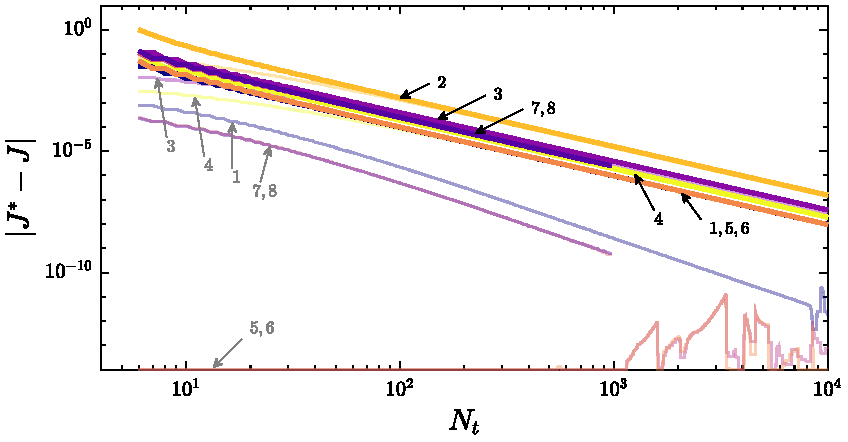
\includegraphics[width=\textwidth]{../ch5/figures/ex2_sens_objective}%
\caption{Objective error.}
\label{fig:ch5:ex2sens:objective}
\end{subfigure}%
\begin{subfigure}{0.5\textwidth}
\centering
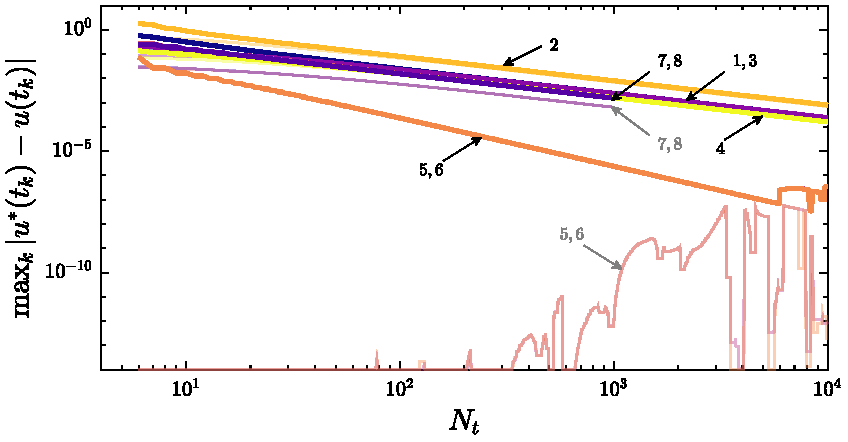
\includegraphics[width=\textwidth]{../ch5/figures/ex2_sens_control}%
\caption{Control error.}
\label{fig:ch5:ex2sens:control}
\end{subfigure}%

\begin{subfigure}{0.5\textwidth}
\centering
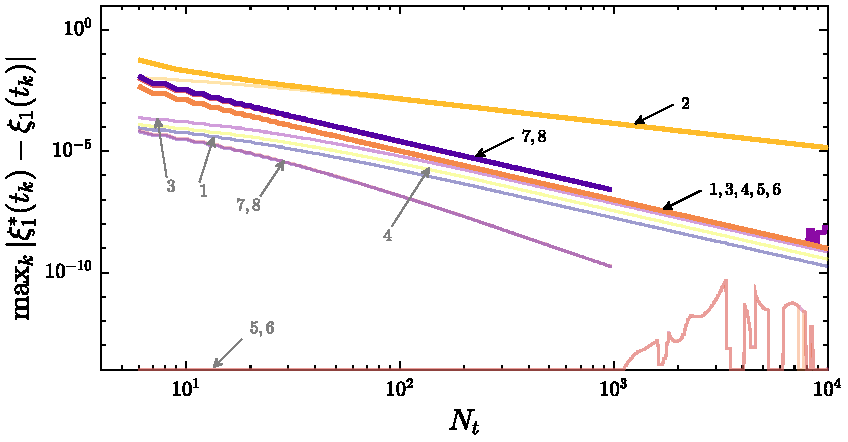
\includegraphics[width=\textwidth]{../ch5/figures/ex2_sens_state_1}%
\caption{$\xi_1$ error.}
\label{fig:ch5:ex2sens:state:1}
\end{subfigure}%
\begin{subfigure}{0.5\textwidth}
\centering
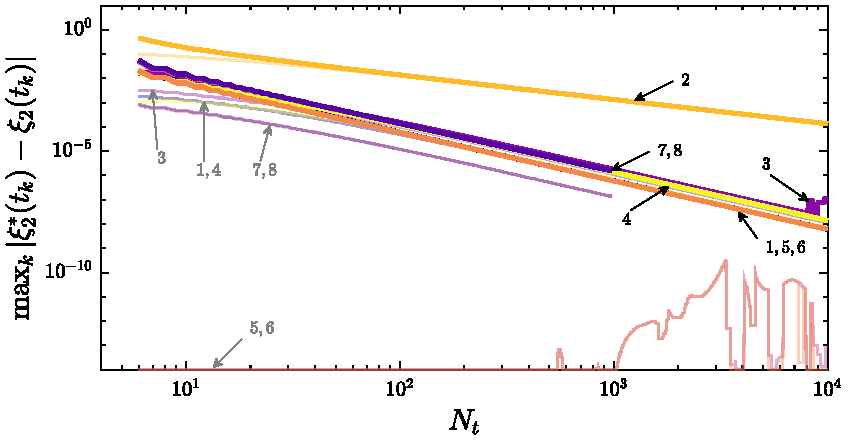
\includegraphics[width=\textwidth]{../ch5/figures/ex2_sens_state_2}%
\caption{$\xi_2$ error.}
\label{fig:ch5:ex2sens:state:2}
\end{subfigure}%

\caption{Numerical results for \nameref{sec:ch5:example2}.}
\label{fig:ch5:ex2sens}
\end{figure}

%-------------------------------------------------------------
\subsection{Example 3} \label{sec:ch5:example3}

%-------------------------------------------------------------
\subsubsection{Description}

For the third example, we will consider the problem on pp.~109--110 of Ref.~\cite{Bryson1975a}:
\begin{subequations}%%
\begin{align}
\min_{u(t)} \quad & \frac{a^2}{2} [ \xi(t_f) ]^2 + \frac{1}{2}\int_{0}^{t_f} u^2 dt \\
\text{subject to:} \quad  & \dot{\xi} = b(t) u \\
& \xi(0) = \xi_0 \\
& \abs{u(t)} \leq 1
\end{align}
\end{subequations}%

\noindent This problem has time-varying matrices, path constraints, and both Lagrange and Mayer terms.
The structure-based problem description for this example is:
\allowdisplaybreaks[1]%
\begin{subequations}%%
\begin{gather}
% Mayer term
\mathcal{M}\xind{1}.\xvar{left} = 5, \quad \mathcal{M}\xind{1}.\xvar{right} = 5, \quad \mathcal{M}\xind{1}.\xvar{matrix} = a^2/2 \\
% Lagrange term
\mathcal{L}\xind{1}.\xvar{left} = 1, \quad \mathcal{L}\xind{1}.\xvar{right} = 1, \quad \mathcal{L}\xind{1}.\xvar{matrix} = 1/2 \\
% dynamics
A = 0, \quad B = b(t) \\
% initial condition
% simple bound
\mathcal{UB}\xind{1}.\xvar{right} = 4, \quad \mathcal{UB}\xind{1}.\xvar{matrix} = \xi_0, \quad
\mathcal{LB}\xind{1}.\xvar{right} = 4, \quad \mathcal{LB}\xind{1}.\xvar{matrix} = \xi_0 \\
\mathcal{UB}\xind{2}.\xvar{right} = 1, \quad \mathcal{UB}\xind{2}.\xvar{matrix} = 1, \quad
\mathcal{LB}\xind{2}.\xvar{right} = 1, \quad \mathcal{LB}\xind{2}.\xvar{matrix} = -1
\end{gather}
\end{subequations}%%
\allowdisplaybreaks[0]%

\noindent The \textsc{Matlab} code is in Sec.~\ref{sec:ex3-code}.

%-------------------------------------------------------------
\subsubsection{Solution}

\begin{figure}
\centering

\begin{subfigure}{0.5\textwidth}
\centering
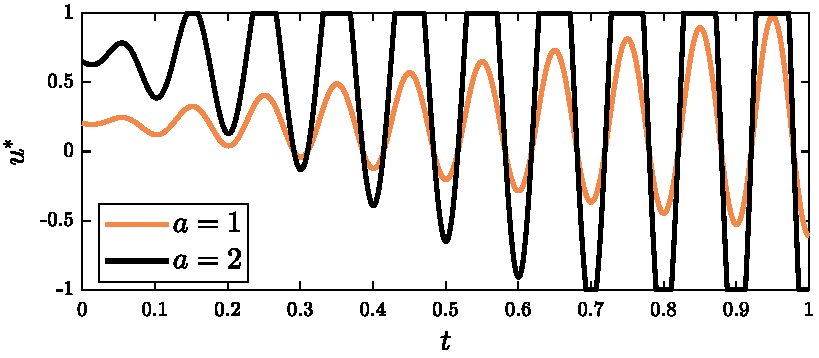
\includegraphics[width=\textwidth]{../ch5/figures/ex3sol-controls}%
\caption{Control.}
\label{fig:ch5:ex3sol:controls}
\end{subfigure}%
\begin{subfigure}{0.5\textwidth}
\centering
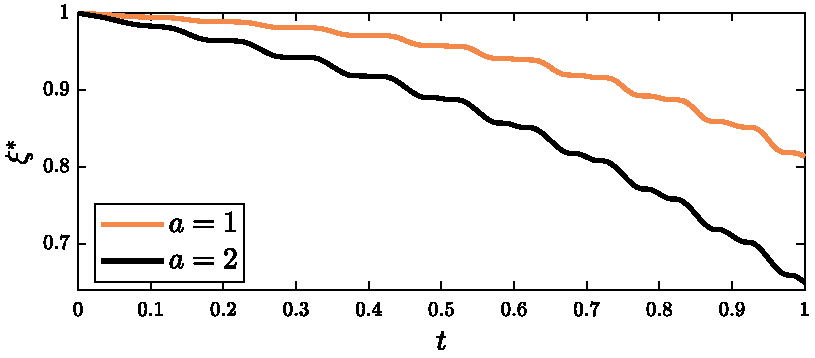
\includegraphics[width=\textwidth]{../ch5/figures/ex3sol-states}%
\caption{State.}
\label{fig:ch5:ex3sol:states}
\end{subfigure}%

\caption{Solutions for \nameref{sec:ch5:example3}.}
\label{fig:ch5:ex3sol}
\end{figure}

The optimal control is:
\begin{align}
u^*(t) &= - \mathrm{sat}\left[ a^2 b(t) \xi(t_f) \right]
\end{align}

\noindent where $\xi(t_f)$ is computed from the implication equation:
\begin{align}
\xi(t_f) &= \xi_0 - \int_0^{t_f} b(t) \mathrm{sat}\left[ a^2 b(t) \xi(t_f) \right] dt 
\end{align}

\noindent The problem parameters used are $t_f = 1$, $\xi_0 = 1$, and $b(t) = t \cos(20 \pi t) - 1/4$.
Both $a = 1$ and $a = 2$ will be tested.
For $a=1$, $\Psi^* = 0.406759$ and $\xi^*(t_f) = 0.813517$.
For $a=2$, $\Psi^* = 1.150647$ and $\xi^*(t_f) = 0.649528$.
The optimal trajectories for control and state for both values of $a$ are shown in Fig.~\ref{fig:ch5:ex3sol}.
With $a=1$, the path constraints are never active, but with $a=2$, the path constraints switch activity frequently. 

%-------------------------------------------------------------
\subsubsection{Numerical Results}

\begin{figure}%
\centering

{\footnotesize Local maximum values (local minimum values are in a thinner, translucent color):}


\includegraphics[width=\textwidth]{../ch5/figures/ex1_sens_legend}%

\vspace{1mm}

\begin{subfigure}{0.5\textwidth}
\centering
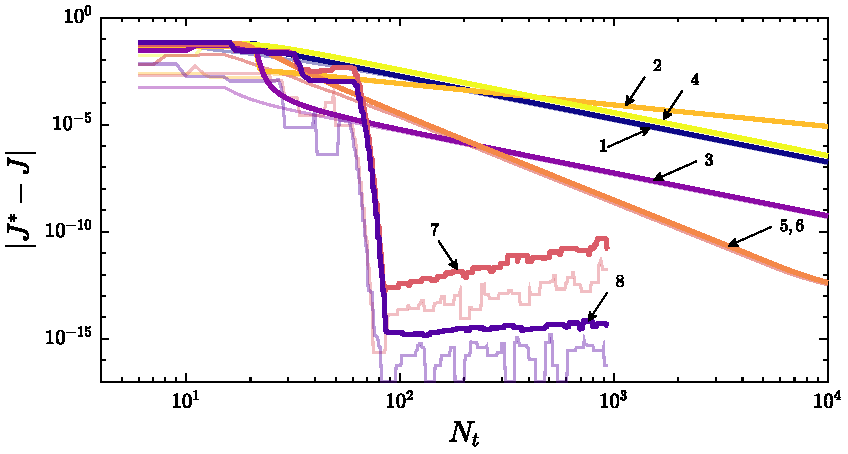
\includegraphics[width=\textwidth]{../ch5/figures/ex3_sens_objective_a1}%
\caption{Objective error with $a=1$.}
\label{fig:ch5:ex3sens:objective:a1}
\end{subfigure}%
\begin{subfigure}{0.5\textwidth}
\centering
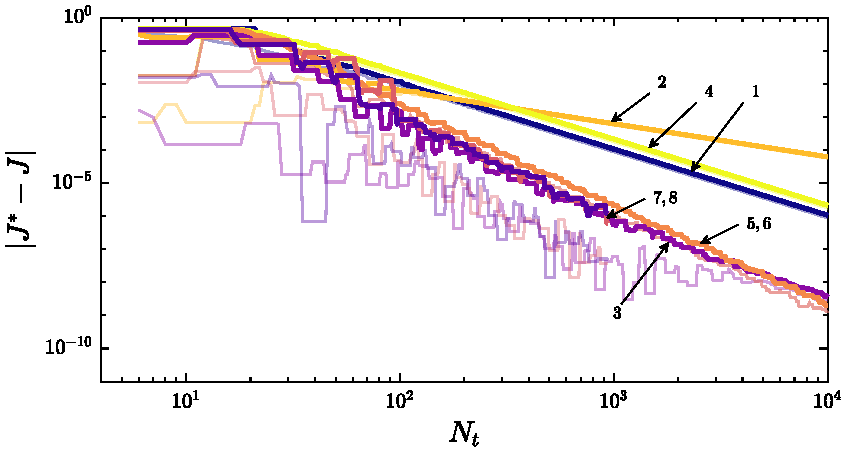
\includegraphics[width=\textwidth]{../ch5/figures/ex3_sens_objective_a2}%
\caption{Objective error with $a=2$.}
\label{fig:ch5:ex3sens:objective:a2}
\end{subfigure}%

\begin{subfigure}{0.5\textwidth}
\centering
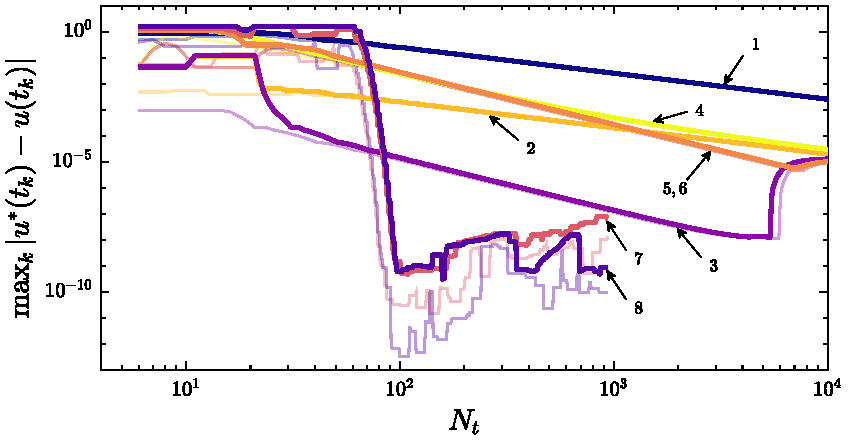
\includegraphics[width=\textwidth]{../ch5/figures/ex3_sens_control_a1}%
\caption{Control error with $a=1$.}
\label{fig:ch5:ex3sens:control:a1}
\end{subfigure}%
\begin{subfigure}{0.5\textwidth}
\centering
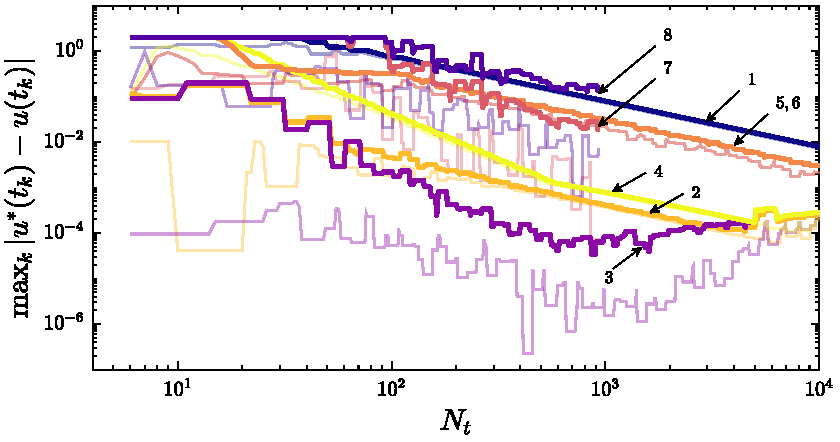
\includegraphics[width=\textwidth]{../ch5/figures/ex3_sens_control_a2}%
\caption{Control error with $a=2$.}
\label{fig:ch5:ex3sens:control:a2}
\end{subfigure}%

\begin{subfigure}{0.5\textwidth}
\centering
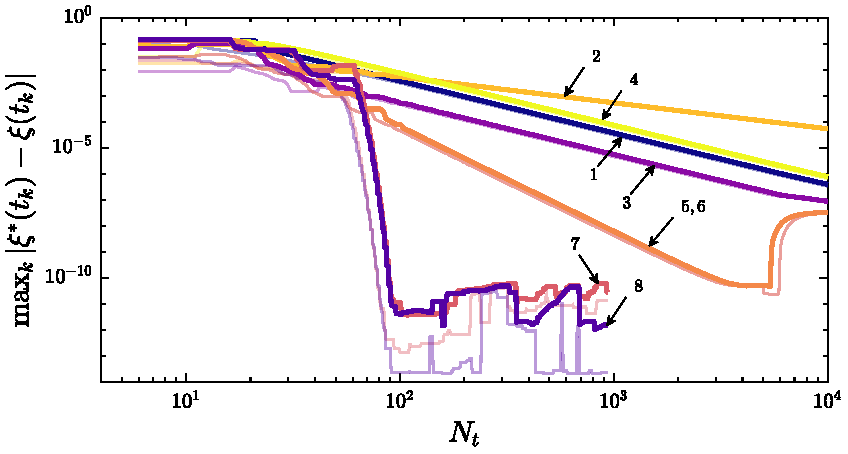
\includegraphics[width=\textwidth]{../ch5/figures/ex3_sens_state_1_a1}%
\caption{State error with $a=1$.}
\label{fig:ch5:ex3sens:state:a1}
\end{subfigure}%
\begin{subfigure}{0.5\textwidth}
\centering
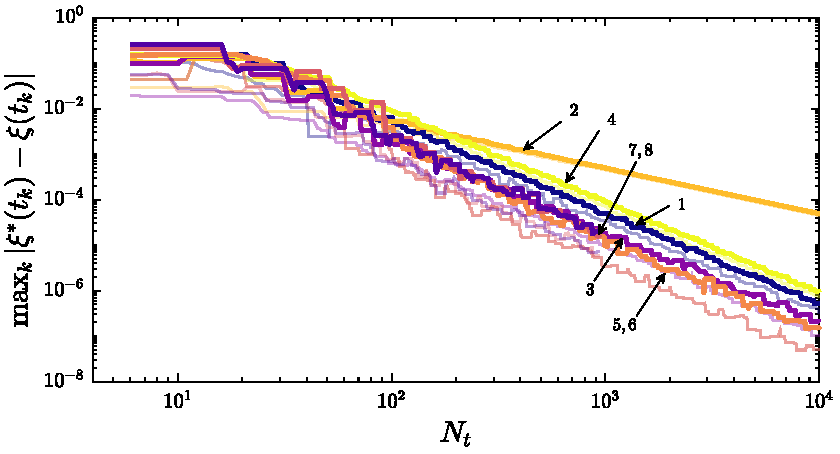
\includegraphics[width=\textwidth]{../ch5/figures/ex3_sens_state_1_a2}%
\caption{State error with $a=2$.}
\label{fig:ch5:ex3sens:state:a2}
\end{subfigure}%

\caption{Numerical results for \nameref{sec:ch5:example3}.}
\label{fig:ch5:ex3sens}
\end{figure}

The convergence results for the eight tested schemes and both values of $a$ are shown in Fig.~\ref{fig:ch5:ex3sens}.
When $a=1$ (where the path constraints are not active), the results are somewhat similar to \nameref{sec:ch5:example1}.
The best methods are the two PS-based schemes (7,8), but unlike the previous example, the gap between them is negligible.
Although the SS-based schemes are converging to the true solution, the ranking of the schemes depends highly on the relative preference between the objective, control, or state errors.
The two CQHS-based schemes have lower state error, but higher control error.
ED-TR-CTR (3) has much lower control error, but higher state error. 
With respect to the objective error, (3) begins with lower error but there is a transition point around $N_t=200$ where (5,6) exhibit less error.
We also see ED-HS-CTR (4) performing worse than (3), differing from the previous examples.

% new paragraph
With $a=2$, the results are quite different with more sporadic convergence behavior (especially for the control).
We observe that (3) is now the best scheme.
Combining the results from both values of $a$, (3) appears to be the best option if high accuracy is required in both problem versions.
These unexpected results might be explained by the fact that there is no $\bm{A}$ in this example (a fairly uncommon property in \lqdo). As a result, this example may prove to be a useful, challenging test problem in the future.
As a result, this example may prove to be a useful, challenging test problem in the future.
Fully understanding these results is left as future work.

%-------------------------------------------------------------
\subsection{Example 4} \label{sec:ch5:example4}

%-------------------------------------------------------------
\subsubsection{Description}

For the fourth example, we will consider the finite-horizon LQR problem in Prob.~(\ref{eq:ch5:lqr}) \cite{Bryson1975a,Liberzon2012a}:%
\begin{subequations}%%
\begin{align}
\min_{\bm{u}(t)} \quad & \left[ \bm{\xi}\tran \bm{M} \bm{\xi} \right]_{t=t_f} + 
\int_{t_0}^{t_f} \left[ \bm{\xi}\tran \bm{Q} \bm{\xi} + \bm{u}\tran \bm{R} \bm{u} \right] dt \\
\text{subject to:} \quad & \dot{\bm{\xi}} = \bm{A} \bm{\xi} + \bm{B} \bm{u} \\
& \bm{\xi}(t_0) = \bm{\xi}_0
\end{align}
\end{subequations}%

\noindent where $\bm{M}$ and $\bm{Q}$ are symmetric positive semidefinite and $\bm{R}$ is symmetric positive definite.
The structure-based problem description for this example is:%
\allowdisplaybreaks[1]%
\begin{subequations}%%
\begin{gather}
% Mayer term
\mathcal{M}\xind{1}.\xvar{left} = 5, \quad \mathcal{M}\xind{1}.\xvar{right} = 5, \quad \mathcal{M}\xind{1}.\xvar{matrix} = \bm{M} \\
% Lagrange term
\mathcal{L}\xind{1}.\xvar{left} = 2, \quad \mathcal{L}\xind{1}.\xvar{right} = 2, \quad \mathcal{L}\xind{1}.\xvar{matrix} = \bm{Q} \\
\mathcal{L}\xind{2}.\xvar{left} = 1, \quad \mathcal{L}\xind{2}.\xvar{right} = 1, \quad \mathcal{L}\xind{2}.\xvar{matrix} = \bm{R} \\
% dynamics
% \bm{A}, \bm{B} \text{ given} \\
% initial condition
\mathcal{UB}\xind{1}.\xvar{right} = 4, \quad \mathcal{UB}\xind{1}.\xvar{matrix} = \bm{\xi}_0, \quad
\mathcal{LB}\xind{1}.\xvar{right} = 4, \quad \mathcal{LB}\xind{1}.\xvar{matrix} = \bm{\xi}_0
\end{gather}
\end{subequations}%%
\allowdisplaybreaks[0]%

\noindent The \textsc{Matlab} code is in Sec.~\ref{sec:ex4-code}.

%-------------------------------------------------------------
\subsubsection{Solution} \label{sec:ch5:ex4:solution}

\begin{figure}
\centering

\begin{subfigure}{0.5\textwidth}
\centering
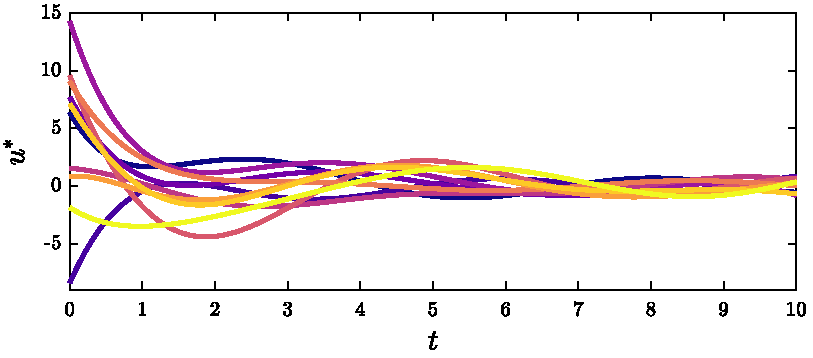
\includegraphics[width=\textwidth]{../ch5/figures/ex4sol-controls}%
\caption{Control.}
\label{fig:ch5:ex4sol:controls}
\end{subfigure}%
\begin{subfigure}{0.5\textwidth}
\centering
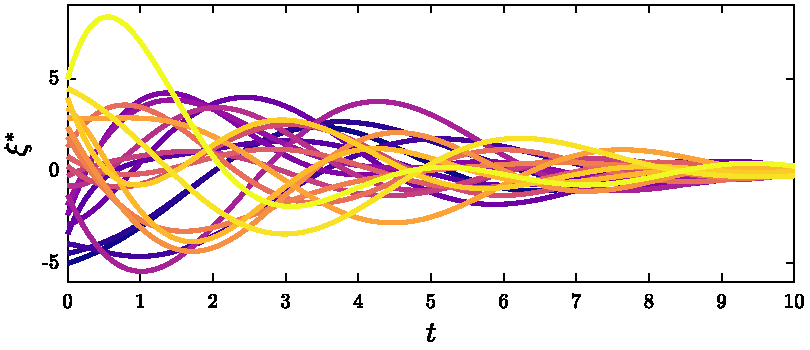
\includegraphics[width=\textwidth]{../ch5/figures/ex4sol-states}%
\caption{States.}
\label{fig:ch5:ex4sol:states}
\end{subfigure}%

\caption{Solution for \nameref{sec:ch5:example4}.}
\label{fig:ch5:ex4sol}
\end{figure}

The optimal control has the following form \cite{Bryson1975a,Liberzon2012a}:
\begin{align}
\bm{u}^* = - \bm{R}^{-1} \bm{B}\tran \bm{P} \bm{\xi}
\end{align}

\noindent where $\bm{P}$ is symmetric positive semidefinite matrix that is a solution to the following differential equation and boundary condition:
\begin{align}
\dot{\bm{P}} = -\bm{Q} - \bm{A}\tran \bm{P} - \bm{P} \bm{A} + \bm{P} \bm{B} \bm{R}^{-1} \bm{B}\tran \bm{P}, \quad \bm{P}(t_f) = \bm{M}
\end{align}

\noindent The specific problem parameters are shown in Sec.~\ref{sec:ex4-code} ($n_\xi = 20$ and $n_u=10$ with generated matrices).
The optimal trajectories for controls and states are shown in Fig.~\ref{fig:ch5:ex4sol}, and were determined by numerically solving the BVP problem with a relative error tolerance at $10^{-10}$.

%-------------------------------------------------------------
\subsubsection{Numerical results}

\begin{figure}%
\centering

{\footnotesize Local maximum values (local minimum values are in a thinner, translucent color):}


\includegraphics[width=\textwidth]{../ch5/figures/ex1_sens_legend}%

\vspace{1mm}

\begin{subfigure}{0.5\textwidth}
\centering
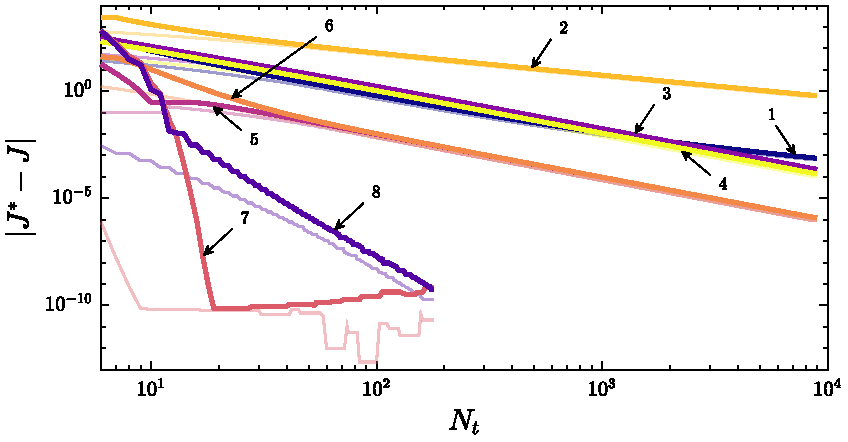
\includegraphics[width=\textwidth]{../ch5/figures/ex4_sens_objective}%
\caption{Objective error.}
\label{fig:ch5:ex4sens:objective}
\end{subfigure}%
\begin{subfigure}{0.5\textwidth}
\centering
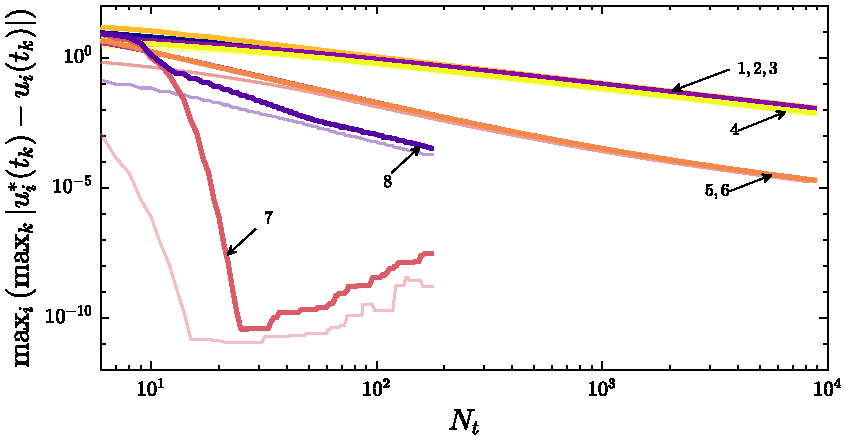
\includegraphics[width=\textwidth]{../ch5/figures/ex4_sens_control}%
\caption{Control error.}
\label{fig:ch5:ex4sens:control}
\end{subfigure}%

\begin{subfigure}{0.5\textwidth}
\centering
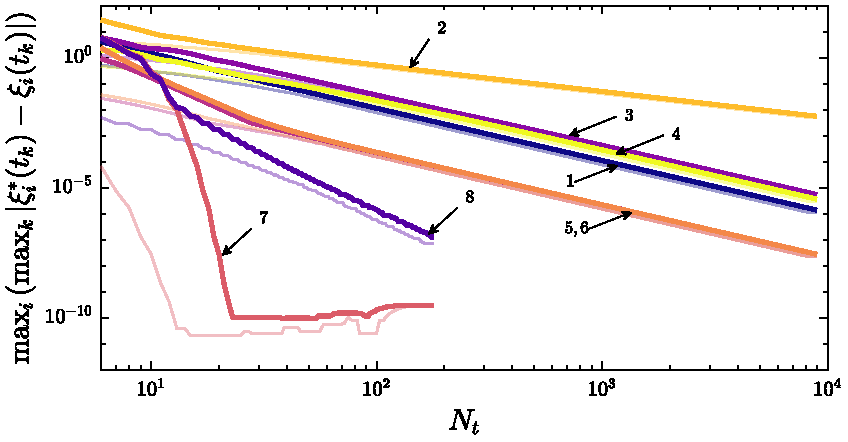
\includegraphics[width=\textwidth]{../ch5/figures/ex4_sens_state_1}%
\caption{State error.}
\label{fig:ch5:ex4sens:state-1}
\end{subfigure}%
\begin{subfigure}{0.5\textwidth}
\centering
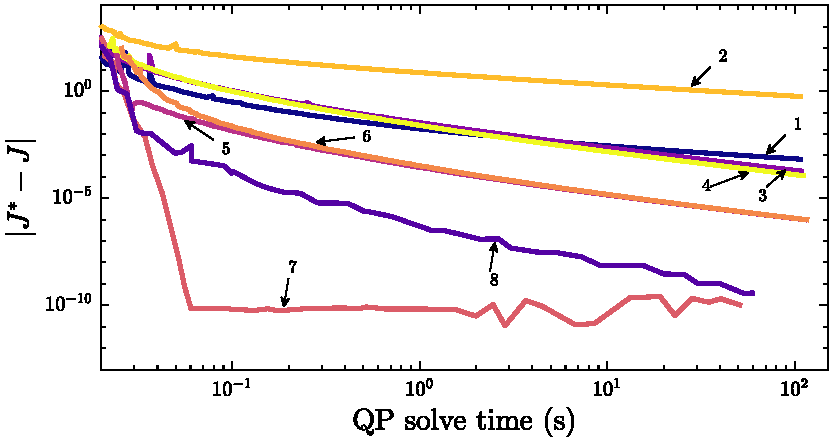
\includegraphics[width=\textwidth]{../ch5/figures/ex4_sens_solve_time}%
\caption{Objective error vs. total \qp{} solve time.}
\label{fig:ch5:ex4sens:solvetime}
\end{subfigure}%

\caption{Numerical results for \nameref{sec:ch5:example4}.}
\label{fig:ch5:ex4sens}
\end{figure}

The convergence results for the eight tested schemes are shown in Fig.~\ref{fig:ch5:ex4sens}.
The numerical results for this example are quite similar to \nameref{sec:ch5:example1} (see Fig.~\ref{fig:ch5:ex1sens}).
The PS-based methods (7,8) performed the best, followed by the CQHS-based methods (5,6). Then was (1,3,4) and finally (1) was the worst again.
The primary discussion point for this example is the efficiency at which the LQR problem was solved.
The objective error vs. total \qp{} solve time is shown in Fig.~\ref{fig:ch5:ex4sens:solvetime}.
LGL-PS-G (7) with $N_t=23$ took only 0.2~s to create and solve the \qp{} with an accuracy in states, controls, and objective value at the tolerance used ($10^{-10}$) when generating the BVP solution in Sec.~\ref{sec:ch5:ex4:solution}.
These results demonstrate that \dt{} approximations of the finite-horizon LQR problem can be a competitive solution strategy.

%-------------------------------------------------------------
\subsection{Example 5} \label{sec:ch5:example5}

%-------------------------------------------------------------
\subsubsection{Description}

The final example is a constructed problem that will help demonstrate some of the problem elements and extensions in Sec.~\ref{sec:ch5:extensions} not seen in the previous examples.
The infinite-dimensional problem formulation is:%
\allowdisplaybreaks[1]%
\begin{subequations}%%
\begin{align}
\min_{\bm{u}(t)} \quad & \int_0^1 \left[ u_1^2/10 + u_2^2/10 + u_1\xi_1 + u_1\xi_2 + 5\left(\xi_2-g(t)\right)^2 \right] dt + \max_{0\leq t\leq 1} \xi_3(t) \\
\text{subject to:} \quad & \dot{\bm{\xi}} = \begin{bmatrix} -1 & 2 & 0 \\ 3 & -4 & 0 \\ 1 & 2 & -1 \end{bmatrix} \bm{\xi} +
\begin{bmatrix} 1 & 0 \\ -1 & 0 \\ 0 & 1/20 \end{bmatrix} \bm{u} \\
& \xi_1(0) = 2, \quad \xi_3(0) = 1/2 \\
& \xi_2(0) - \xi_2(1) = 0 \\
& \int_0^1 \xi_1(t) dt = 0 \\
& -\xi_1(t) + u_2(t)/12 \leq 0 \\
& \xi_2(t) \leq g(t) \\
& \abs{u_2} \leq 10 
\end{align}
\end{subequations}%%
\allowdisplaybreaks[0]%

\noindent where 
$5\left(\xi_2-g(t)\right)^2$ is an output tracking term (resulting in time-varying quadratic, linear, and constant objective function terms, see Sec.~\ref{sec:ch5:output}),
$\max\xi_3(t)$ is a min-max objective term (that will be approximated with a parameter, see Sec.~\ref{sec:ch5:minmax:objective}),
$\xi_2(0) - \xi_2(1) = 0$ is a periodic constraint (that will be implemented as a linear equality constraint),
$\int_0^1 \xi_1(t) dt = 0$ is an integral constraint (which will be approximated with an additional state, see Sec.~\ref{sec:ch5:integral:constraints}),
$-\xi_1(t) + u_2(t)/12 \leq 0$ is a mixed control-state path constraint,
$\xi_2(t) \leq g(t) $ is a time-varying simple bound,
and
$\abs{u_2} \leq 10 $ is a linear absolute value constraint (that will be implemented with two constraints, see Sec.~\ref{sec:ch5:absolute:values}).
For brevity, the structure-based implementation is only shown in the \textsc{Matlab} code in Sec.~\ref{sec:ex5-code}. 

%-------------------------------------------------------------
\subsubsection{Solution}

This example, like many \lqdo{} problems, does not have a straightforward solution, so we can instead use \dt{} to obtain an approximate solution.
Here we set $g(t) = \sin(2 \pi t) +1/2$.
The optimal trajectories for the states and controls are shown in Fig.~\ref{fig:ch5:ex5sens} along with the trajectories for the integral and mixed control-state constraints.
This solution was found using ED-HS-CQHS (5) with 5,000 node points and $\Psi^*=6.368153$.
All constraints are satisfied, and all the path constraints enter and exit activity during the time horizon.

\begin{figure}
\centering

\begin{subfigure}{0.5\textwidth}
\centering
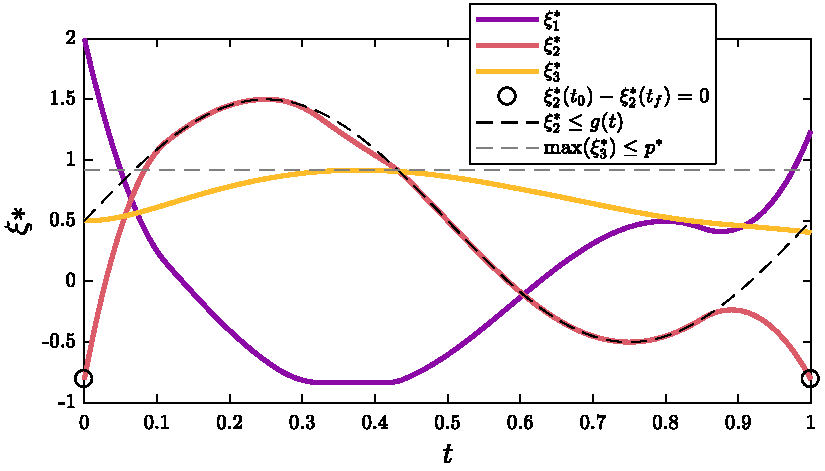
\includegraphics[width=\textwidth]{../ch5/figures/ex5sol-states}%
\caption{States.}
\label{fig:ch5:ex5sol:states}
\end{subfigure}%
\begin{subfigure}{0.5\textwidth}
\centering
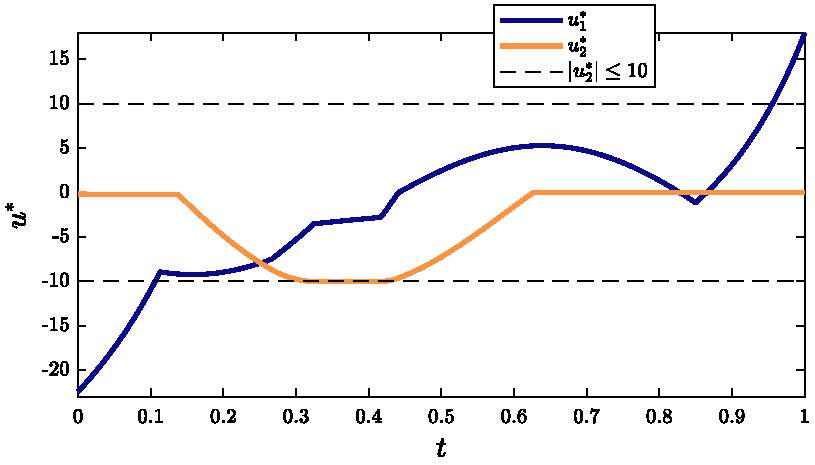
\includegraphics[width=\textwidth]{../ch5/figures/ex5sol-controls}%
\caption{Controls.}
\label{fig:ch5:ex5sol:controls}
\end{subfigure}%

\begin{subfigure}{\textwidth}
\centering
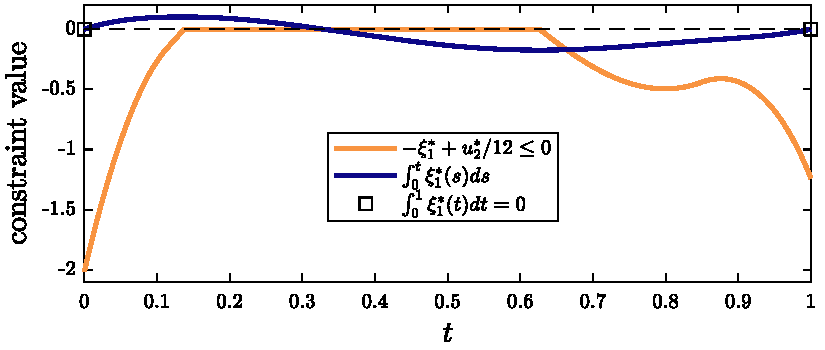
\includegraphics[width=0.5\textwidth]{../ch5/figures/ex5sol-other}%
\caption{Integral and mixed state-control path constraints.}
\label{fig:ch5:ex5sol:other}
\end{subfigure}%

\caption{Solution for \nameref{sec:ch5:example5}.}
\label{fig:ch5:ex5sens}
\end{figure}

\section{Future Work} \label{sec:ch5:future:work}

The proposed \apgp{} and unified \lqdo{} problem description can provide a strong basis for a number of future developments that could improve the effectiveness and the user experience.

%-----------------------------------------------------------
\subsection{Multiple-Interval Pseudospectral Methods and Multiphase Problems} \label{sec:ch5:multipleinterval}

The current implementation of the PS methods utilizes a single interpolating polynomial over the entire time horizon to approximate the states and controls.
Since the interpolating polynomials are continuous basis functions, approximated quantities at the time values between node points may contain significant inaccuracy with any of discontinuity or non-smoothness imposed in the optimal function shape.
In addition, since the particular PS method requires a specific form of the mesh (e.g.,~LGL or CGL meshes), which is stretched in the middle range, having enough resolution at certain location enforces excessive resolution in both end regions.

These problems could be addressed by implementing multiple intervals in our computational domain \cite{Herber2015a, Darby2009b, Patterson2014a}.
Each interval in the time horizon would contain an interpolating polynomial and continuity between the states would be ensured with the following continuity constraint:
\begin{align} \label{eq:ch5:continuity}
\bm{\xi}^{(i-1)}(t^{(i-1)}_f) = \bm{\xi}^{(i)}(t^{(i)}_0), \qquad \text{where:  } t^{(i-1)}_f = t^{(i)}_0
\end{align}

\noindent which is a linear equality constraint; thus, is possible in \lqdo.
This multiple-interval approach can also be implemented along with the \textit{hp}-adaptive mesh refinement technique described the following section \cite{Gong2008a, Darby2009b, Fujikawa2014a}.

% new paragraph
Conceptually similar, multiphase problems could be proposed \cite{Patterson2014a}.
In a multiphase problem, various continuity constraints (which need not be the same form as Eqn.~(\ref{eq:ch5:continuity})) are present to ensure consistency across the phases.
The problem elements between the phases may be different (e.g.,~different constraints present or the dynamics change).
Unlike the multiple-interval approximation method, multiphase problems can be solved with all the methods listed here.

%-----------------------------------------------------------
\subsection{Mesh Refinement} \label{sec:ch5:meshrefinement}

The accuracy assessments in Sec.~\ref{sec:ch5:examples} were performed on problems with known exact solutions.
However, for many \lqdo{} problems, such solutions are unavailable (and is a primary reason for using \dt{}).
Resolution of mesh nodes and location of each node affect the overall solution accuracy and mesh refinement (iteratively solving the problem on a specific mesh and then updating the mesh with changes in the mesh resolution and node locations) is a viable technique for obtaining high accuracy solutions to continuous-time dynamic optimization problems \cite{Betts1998b, Darby2009b}.
Such techniques are particularly useful when there is discontinuity or non-smoothness in the solution (e.g.,~when path constraints change activity).

% new paragragh
There are two common types of mesh refinement: \textit{h}- and \textit{p}-adaptive methods \cite{zhao2017a}.
For the SS methods, the \textit{h}-adaptive methods could be employed to minimize the local and global discretization error \cite{Betts1998b, Betts2000a, Jain2008a}.
For the multiple-interval PS methods, the combined \textit{hp}- or \textit{ph}-adaptive methods could be applied to get the benefit of spectral convergence within local time interval while accommodating discontinuities between neighboring time intervals \cite{Darby2009b, Darby2011a, Fujikawa2014a, Patterson2015a}.
Since mesh refinement is performed offline (not when solving the \qp), it can readily be incorporated into the \apgp.

%-----------------------------------------------------------
\subsection{Costate Approximation and First-Order Necessary Conditions}

Alternative methods to \dt{} are the indirect methods which derive a set of first-order necessary conditions for optimality for the DO problem (e.g.,~these conditions were used to derive the BVP in \nameref{sec:ch5:example4}).
Even though there are a number of challenges associated with using indirect methods \cite{Betts2010a, Biegler2010a, Bryson1975a, Herber2014a}, it still can be useful to utilize the concepts from the indirect methods.
For example, the costate variables are the time-varying multipliers associated with the dynamics in the augmented Hamiltonian.
Similar to the states and controls, these have optimal values as well.
Errors in the costates can be assessed in a similar manner to states and controls to help determine the convergence properties of each of the methods.
In addition, computing the Hamiltonian given the \dt{} solution can help verify the quality of the solution.

% new paragraph
Determining the values of the costates and other multipliers is done through a mapping from the \glsfoo[noindex]{KKT} multipliers of the finite-dimensional optimization problem \cite{Garg2011a, Francolin2014a}.
Estimations of costate have been studied for finite and infinite time horizons with direct optimal control methods \cite{Garg2011a, Francolin2014a, Darby2011b, Schori2015a}.
Approximating costates with discontinuous trajectories requires a jump condition between discontinued segments \cite{Darby2011b, Schori2015a} and is especially important when the multiple intervals are considered for problems with discontinuous dynamic behavior, described in Sec.~\ref{sec:ch5:multipleinterval}.
Various dynamic optimization software tools have provided these estimates \cite{Patterson2014a, Becerra2015a}.
Computing these estimates for \lqdo{} would be no different than the general NLDO problems and might, in fact, be simpler due to the structured form of the objective and dynamics.

%-----------------------------------------------------------
\subsection{Additional Methods} \label{sec:ch5:add:methods}

A large number of methods to construct the defect constraints were listed in Sec.~\ref{sec:ch5:defects}.
Only a small subset of these available methods have been implemented, and it remains future work to implement (as long as they are order-maintaining methods) and assess the effectiveness of these methods in \lqdo.
Different quadrature schemes may also be considered, such as  the true HS quadrature scheme that uses Eqn.~(\ref{eq:ch5:xhs}).

%-----------------------------------------------------------
\subsection{Customized {QP} Solvers}

The numerical results in Sec.~\ref{sec:ch5:examples} were found using one solver available in \textsc{Matlab}.
There are a number of other \qp{} solvers available (e.g.,~\textsc{ooqp} \cite{Gertz2003a} and \textsc{cvx} \cite{Grant2008a}) that may be more suitable for this class of problems (both in computational efficiency and convergence).
An effective solver should be able to handle large matrices, the specific sparsity patterns, and ill-conditioned matrices.
Perhaps a custom \qp{} solver could be created that handles this type of ill-conditioned problems \cite{Torsti1972a, Gould2000a, Donoghue2013a, Ghadimi2015a}.
Some recent \qp{} methods have used \lqdo{} problems with specific \dt{} methods as one of their test problems \cite{ Donoghue2013a, Ghadimi2015a}.

% new paragraph
Some of these numerical difficulties were illustrated in the results using the LGL-PS-G (7) scheme.
This scheme typically exhibited a tendency of divergence after exponential convergence up to a specific polynomial order.
A rapid growth of condition number along with a growth of the differential operator order causes this instability, which makes the problem nonconvex and may sacrifice the expected spectral accuracy of the solution \cite{Wang2014a, Trefethen1987a}.

%-----------------------------------------------------------
\subsection{Scaling}

It has been established that properly-scaled optimization problems are easier to solve than a poorly-scaled problem \cite{Rao2010a}.
In general, this is embodied by the constraints and optimization variables being close to $\mathcal{O}(1)$ \cite{Gill1981a}.
Affine transformations of both the optimization variables and time horizon can be utilized to accomplish this task \cite{Herber2017c, Rao2010a}.
An example of this type of transformation is the similarity transform applied to linear systems \cite{Chen1999a}.
The constraints can be directly scaled by the row norms of the matrices \cite{Rao2010a}. 
Systematic preconditioning methods have been developed for linear constraints \cite{Bergamaschi2004a, Benzi2002a}.
Properly-scaled defect constraints are particularly important to ensure the accuracy of the approximation \cite{Herber2017c}.
Using these concepts, among other techniques, automatic scaling procedures have been developed for DO problems \cite{Rao2010a}.

%-----------------------------------------------------------
\subsection{Quadratically-Constrained Quadratic Programs} \label{sec:ch5:QCQP}

A more general class of optimization problems that includes {\qp}s as a special case are \glsfirst{QCQP} \cite{Boyd2009a}.
The objective is the same as in Eqn.~(\ref{eq:ch5:qpH}), but we now include constraints with up to quadratic dependence:%
\begin{subequations} \label{eq:ch5:QCQP}
\begin{align}
\frac{1}{2}\mathbf{X}\tran\mathbf{P}_{e}\mathbf{X}  + \mathbf{A}_{e}\mathbf{X} = \mathbf{B}_{e} \\
\frac{1}{2}\mathbf{X}\tran\mathbf{P}_{i}\mathbf{X}  + \mathbf{A}_{i}\mathbf{X} \leq \mathbf{B}_{i}
\end{align}
\end{subequations}%

\noindent In general, a QCQP is an NP-hard problem \cite{So2011a}.
However, if all inequality constraints are convex and only linear equality constraints are present, then the QCQP can be solved with semidefinite programming or second-order cone programming \cite{Boyd2009a}.
Modifying the algorithms in Sec.~\ref{sec:ch5:algorithm} to generate QCQPs and understanding the structural properties of the generated matrices is future work. 
There are many interesting items that could be represented with QCQPs, including quadratic terms in the dynamics \cite{Sun2016a}, MTPs, simple co-design problems (e.g.,~$\dot{\xi} = k \xi$, where $k$ is also an optimization variable) \cite{Herber2017b}, power and energy terms (e.g.,~$\xi u$) \cite{Herber2014a, Faedo2017a}, and the conversion of quadratic Lagrange terms to Mayer form as quadratic equality constraints (discussed in Sec.~\ref{sec:ch5:integral:constraints}).

%-------------------------------------------------------------------
\section{Summary} \label{sec:ch5:conclusion}

In this chapter, a unified framework for solving general linear-quadratic dynamic optimization (\lqdo{}) problems was proposed.
This class of dynamic optimization problems contains problem elements such as a linear nonhomogeneous differential equation, quadratic objective function terms, and additional linear constraints where the optimization variables include the controls, states, parameters, initial state values, and final states values.

% new paragraph
A class of numerical methods known as direct transcription (\dt) was utilized to find approximate solutions to the \lqdo{} problem.
The \dt{} methods parameterize both the state and control trajectories and include them as optimization variables. 
A large number of equality constraints (termed defect constraints) are used to ensure feasible dynamics.
Both pseudospectral (PS) and single-step (SS) methods are utilized to construct the defect constraints.
A variety of SS methods are implemented including Euler forward (EF), trapezoidal rule (TR), Hermite-Simpson (HS),  4th-order classical Runge-Kutta (RK4), and zero-order hold (ZOH).
HS and RK4 are frequently utilized on NLDO problems, but rarely with \lqdo{}.
ZOH is a commonly used method, particularly within the MPC framework.
A number of quadrature schemes are implemented including a new composite quadratic Hermite-Simpson (CQHS) method.
This method is derived in a similar manner as the composite HS method, but uses linear interpolation between node points for each term in the quadratic objective function.

% new paragraph
An automated problem generation procedure (\apgp) is fully outlined that makes it relatively straightforward to obtain a \dt{} solution to an \lqdo{} problem.
A structure-based scheme is used to represent the problem.
The algorithms for efficiently generating the sequences that define the sparse matrices is also described.
Full \textsc{Matlab} codes are available at Ref.~\cite{github-dt-qp-project}.
Five examples are shown to demonstrate the efficacy of the \apgp.
Including a variety of \dt{} methods allowed for direct comparisons between the methods.
The PS-based methods had extremely fast convergence in problems with no path constraints, and had a smooth optimal solution in general.
When the nonsmoothness was present in the optimal solutions, the higher-order SS methods performed better, with the HS and RK4 being the best.
The CQHS-based methods generally performed as good as or better than the other SS methods, demonstrating the relative effectiveness of the new quadrature scheme.

% new paragraph
A number of extensions are described including integral constraints, min-max objectives, absolute values, output tracking, control rate constraints, and polyhedra constraints, demonstrating that a diverse set of problems fit under the \lqdo{} framework.
There are a number of methods and features that can be implemented in the future including multiple-interval PS methods, multiphase problems, mesh refinement, costate approximation, additional defect and quadrature methods, customized \qp{} solvers, scaling, and quadratically-constrained {\qp}s.